\documentclass{article}

\usepackage{tikz}
\usetikzlibrary{external}
\usetikzlibrary{decorations.pathmorphing}
\usetikzlibrary{decorations.markings}
\usetikzlibrary{shapes.arrows}
\usetikzlibrary{arrows}

\usetikzlibrary{positioning,fit,calc}
\usetikzlibrary{arrows.meta}
\usetikzlibrary{calc,fadings,decorations.pathreplacing}
%\usetikzlibrary{arrows.spaced}
\usetikzlibrary{decorations.pathmorphing}

\usepackage[compat=1.1.0]{tikz-feynman}

\usepackage{varwidth}
\usepackage{epstopdf}
\usepackage{amssymb}
\usepackage{relsize}

\tikzset{external/system call={lualatex
      \tikzexternalcheckshellescape -halt-on-error -interaction=batchmode
-jobname "\image" "\texsource"}}
%\tikzset{external/force remake}
\tikzexternalize % activate!

\begin{document}


\begin{figure}
\begin{center}
   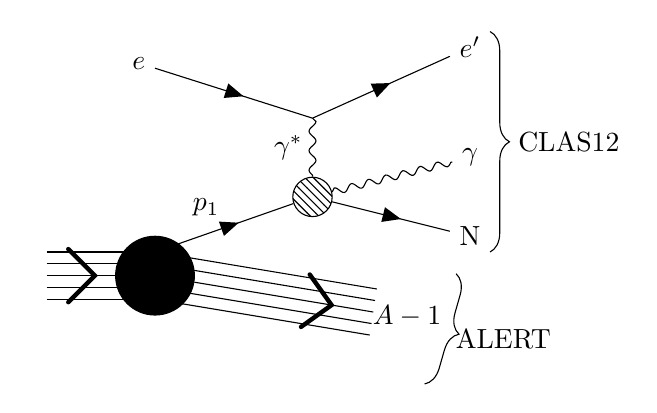
\begin{tikzpicture}
      \begin{feynman}
         \vertex                                            (n0) {};
         \vertex[large, blob, fill=black,right=1.5cm of n0] (n1) {};

         % incoming A nucleons
         \vertex[above = 0.15cm of n0]  (n01){~};
         \vertex[above = 0.30cm of n0]  (n02){~};
         \vertex[above = 0.45cm of n0]  (n03){~};
         \vertex[below = 0.15cm of n0]  (n04){~};
         \vertex[below = 0.30cm of n0]  (n05){~};
         \vertex[below = 0.45cm of n0]  (n06){~};

         \vertex[above = 0.15cm of n1]  (n11){~};
         \vertex[above = 0.30cm of n1]  (n12){~};
         \vertex[above = 0.45cm of n1]  (n13){~};
         \vertex[below = 0.15cm of n1]  (n14){~};
         \vertex[below = 0.30cm of n1]  (n15){~};
         \vertex[below = 0.45cm of n1]  (n16){~};

         \vertex[below right=0.5cm and 3.0cm of n1]            (n2) {};
         %\vertex[label={[label distance=0.2cm]-130:label},blob, fill=black, 

         \vertex[below right=0.5cm and 3.0cm of n11]  (n21) {};
         \vertex[below right=0.5cm and 3.0cm of n12]  (n22) {};
         \vertex[below right=0.5cm and 3.0cm of n13]  (n23) {};
         \vertex[below right=0.5cm and 3.0cm of n14]  (n24) {};
         \vertex[below right=0.5cm and 3.0cm of n15]  (n25) {};
         \vertex[below right=0.5cm and 3.0cm of n16]  (n26) {};

         \vertex[below right=0.5cm and 1.5cm of n2]      (n3) {};

         %dvcs vertex
         \vertex[small, blob, above right=1.0cm and 2.0cm of n1] (a0) {};

         % e,e'gamma vertex 
         \vertex[above=1.0cm of a0]                  (q0);

         \vertex[below right=0.5cm and 2.0cm of a0]  (a1) {N};
         \vertex[above=1.0cm of a1]                  (q1){\(\gamma\)};

         % electron
         \vertex[above left=0.5cm and 2.0cm of q0]  (e0) {\(e\)};
         \vertex[above=1.4 of q1]   (e1) {\(e^{\prime}\)};

         \diagram*{
            (e0) -- [fermion] (q0) -- [fermion] (e1),
            (n12) -- [fermion, edge label=\(p_1\)] (a0) -- [fermion] (a1),
            (a0) -- [photon, edge label = \(\gamma^{*}\)] (q0),
            (q1) -- [photon] (a0),
            (n01) --  (n11)  --  (n21),
            (n02) --  (n12)  --  (n22),
            %(n03) --  (n13) --  (n23),
            (n04) --  (n14)  --  (n24),
            (n05) --  (n15)  --  (n25),
            %(n06) --  (n16) ,
            (n0) -- [plain,arrow size=6pt, postaction={decorate}, 
            decoration={markings, mark=at position 0.75 with 
         {\arrow[scale=4]{angle 90}}}] (n1) --
         [plain,arrow size=6pt, postaction={decorate}, decoration={markings, 
         mark=at position 0.75 with {\arrow[scale=4]{angle 90}}}] (n2),
         };
         \draw[fill,white,rotate=-9] ($(n2.west)-(0.10cm,0.35cm)$) rectangle 
         ($(n2.west)+(0.10cm,0.35cm)$);
         \vertex[below right=0.01cm and 0.2cm of n2]      (pminus1) {$A-1$};

         % alert detection
         \draw [decoration={brace,amplitude=7pt}, decorate]
         ($(n2.north east)+(0.7cm,0.4cm)$) -- ++(-0.4cm,-1.4cm);
         \node[] at ($(n2.east)+(1.3cm,-0.3cm)$) {ALERT};

         % CLAS12 detection
         \draw [decoration={brace,amplitude=7pt}, decorate]
         ($(e1.east)+(0.0cm,0.2cm)$) -- ++(-0.0cm,-2.8cm);
         \node[] at ($(e1.east)+(1.0cm,-1.2cm)$) {CLAS12};

      \end{feynman}
   \end{tikzpicture}
\end{center}
\caption{figure0.pdf}
\end{figure}

\begin{figure}
\begin{center}
   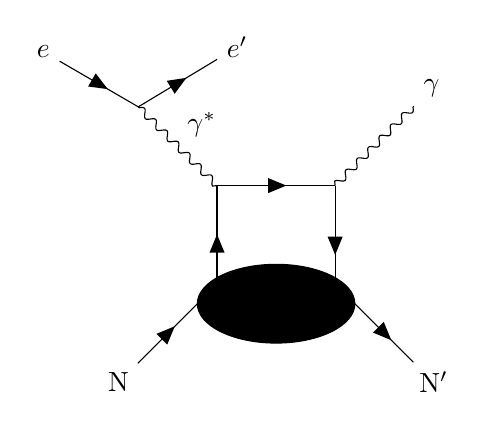
\begin{tikzpicture}
      \begin{feynman}
         \vertex (p1) at (0,0) {N};
         \vertex[above right=1cm and 2.0cm of p1] (a2) { };
         \vertex[below right=1cm and 2.0cm of a2] (p2) {N\(^{\prime}\)};

         \vertex[above left =0.00cm and 1.00cm of a2] (a20);
         \vertex[above left =0.00cm and 0.75cm of a2] (a21);
         \vertex[above left =0.25cm and 0.50cm of a2] (a22);
         \vertex[above left =0.25cm and 0.25cm of a2] (a23);
         \vertex[above right=0.25cm and 0.25cm of a2] (a24);
         \vertex[above right=0.25cm and 0.50cm of a2] (a25);
         \vertex[above right=0.00cm and 0.75cm of a2] (a26);
         \vertex[above right=0.00cm and 1.00cm of a2] (a27);

         \vertex[above =1.5cm of a21] (q0);
         \vertex[above =1.5cm of a26] (q1);


         \vertex[above left =1cm and 1cm of q0] (e0);
         \vertex[above right=1cm and 1cm of q1] (e1){\(\gamma \)};

         \vertex[above left =0.5cm and 1cm of e0] (ee0){\(e\)};
         \vertex[above right=0.5cm and 1cm of e0] (ee1){\(e^{\prime}\)};

         \draw[fill,black] (a2) ellipse (1cm and 0.5cm);
         \diagram* {
            (ee0) -- [fermion] (e0)-- [fermion] (ee1),
            (p1) -- [fermion] (a20),
            (a27) -- [fermion] (p2),
            (a21) -- [fermion] (q0) -- [fermion](q1) -- [fermion](a26),
            (e0) -- [photon, edge label=\(\gamma^{*} \)] (q0),
            (e1) -- [photon] (q1),
         };
      \end{feynman}
   \end{tikzpicture}
\end{center}
\caption{figure1.pdf}
\end{figure}


\begin{figure}
\begin{center}
   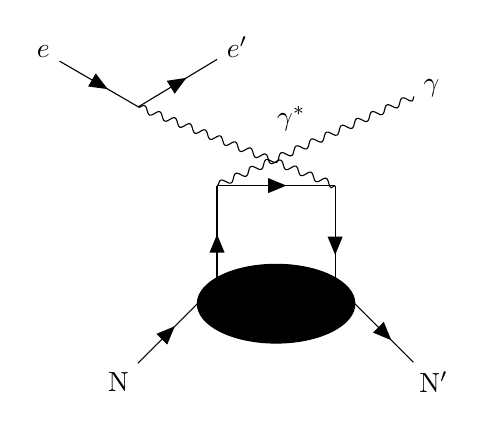
\begin{tikzpicture}
      \begin{feynman}
         \vertex (p1) at (0,0) {N};
         \vertex[above right=1cm and 2.0cm of p1] (a2) { };
         \vertex[below right=1cm and 2.0cm of a2] (p2) {N\(^{\prime}\)};

         \vertex[above left =0.00cm and 1.00cm of a2] (a20);
         \vertex[above left =0.00cm and 0.75cm of a2] (a21);
         \vertex[above left =0.25cm and 0.50cm of a2] (a22);
         \vertex[above left =0.25cm and 0.25cm of a2] (a23);
         \vertex[above right=0.25cm and 0.25cm of a2] (a24);
         \vertex[above right=0.25cm and 0.50cm of a2] (a25);
         \vertex[above right=0.00cm and 0.75cm of a2] (a26);
         \vertex[above right=0.00cm and 1.00cm of a2] (a27);

         \vertex[above =1.5cm of a21] (q0);
         \vertex[above =1.5cm of a26] (q1);

         \vertex[above left =1cm and 1cm of q0] (e0);
         \vertex[above right=1cm and 1cm of q1] (e1){\(\gamma \)};

         \vertex[above left =0.5cm and 1cm of e0] (ee0){\(e\)};
         \vertex[above right=0.5cm and 1cm of e0] (ee1){\(e^{\prime}\)};

         \draw[fill,black] (a2) ellipse (1cm and 0.5cm);
         \diagram* {
            (ee0) -- [fermion] (e0)-- [fermion] (ee1),
            (p1) -- [fermion] (a20),
            (a27) -- [fermion] (p2),
            (a21) -- [fermion] (q0) -- [fermion](q1) -- [fermion](a26),
            (e0) -- [photon] (q1),
            (q0) -- [photon, edge label=\(\gamma^{*} \)] (e1),
         };
      \end{feynman}
   \end{tikzpicture}
\end{center}
\caption{figure2.pdf}
\end{figure}

\begin{figure}
\begin{center}
   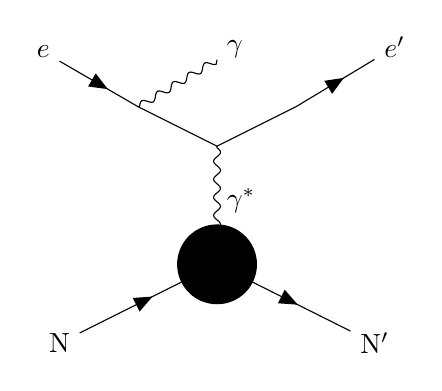
\begin{tikzpicture}
      \begin{feynman}
         \vertex (p1) at (0,0) {N};
         \vertex[above right=1cm and 2.0cm of p1] (a2) { };
         \vertex[below right=1cm and 2.0cm of a2] (p2) {N\(^{\prime}\)};

         \vertex[above left =0.00cm and 1.00cm of a2] (a20);
         \vertex[above left =0.00cm and 0.75cm of a2] (a21);
         \vertex[above left =0.25cm and 0.50cm of a2] (a22);
         \vertex[above left =0.25cm and 0.25cm of a2] (a23);
         \vertex[above right=0.25cm and 0.25cm of a2] (a24);
         \vertex[above right=0.25cm and 0.50cm of a2] (a25);
         \vertex[above right=0.00cm and 0.75cm of a2] (a26);
         \vertex[above right=0.00cm and 1.00cm of a2] (a27);

         \vertex[above =1.5cm of a2] (q0);

         \vertex[above left =0.5cm and 1cm of q0] (e01);
         \vertex[above left =1.0cm and 2cm of q0] (e0){\(e\)};
         \vertex[above right=1.0cm and 2cm of q0] (e1){\(e^{\prime}\)};
         \vertex[above right=0.5cm and 1cm of q0] (e11);

         \vertex[above right=0.5cm and 1.0cm of e01] (q1) {$\gamma$};

         \draw[fill,black] (a2) ellipse (0.5cm and 0.5cm);

         \diagram* {
            (p1) -- [fermion] (a2),
            (a2) -- [fermion] (p2),
            (e0) -- [fermion] (e01) -- [plain] (q0) -- [plain] (e11) -- 
            [fermion] (e1),
            (q0) -- [photon, edge label = \(\gamma^{*}\)] (a2),
            (e01) -- [photon] (q1),
         };
      \end{feynman}
   \end{tikzpicture}
\end{center}
\caption{figure2.pdf}
\end{figure}

\begin{figure}
\begin{center}
   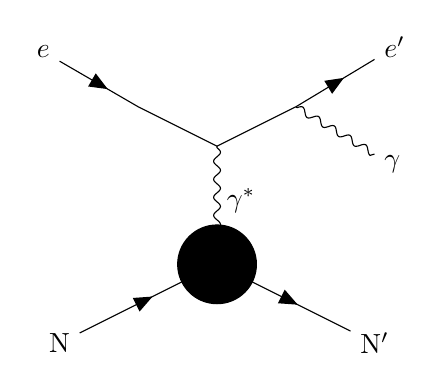
\begin{tikzpicture}
      \begin{feynman}
         \vertex (p1) at (0,0) {N};
         \vertex[above right=1cm and 2.0cm of p1] (a2) { };
         \vertex[below right=1cm and 2.0cm of a2] (p2) {N\(^{\prime}\)};

         \vertex[above left =0.00cm and 1.00cm of a2] (a20);
         \vertex[above left =0.00cm and 0.75cm of a2] (a21);
         \vertex[above left =0.25cm and 0.50cm of a2] (a22);
         \vertex[above left =0.25cm and 0.25cm of a2] (a23);
         \vertex[above right=0.25cm and 0.25cm of a2] (a24);
         \vertex[above right=0.25cm and 0.50cm of a2] (a25);
         \vertex[above right=0.00cm and 0.75cm of a2] (a26);
         \vertex[above right=0.00cm and 1.00cm of a2] (a27);

         \vertex[above =1.5cm of a2] (q0);

         \vertex[above left =0.5cm and 1cm of q0] (e01);
         \vertex[above left =1.0cm and 2cm of q0] (e0){\(e\)};
         \vertex[above right=1.0cm and 2cm of q0] (e1){\(e^{\prime}\)};
         \vertex[above right=0.5cm and 1cm of q0] (e11);

         \vertex[below right=0.5cm and 1.0cm of e11] (q1) {$\gamma$};

         \draw[fill,black] (a2) ellipse (0.5cm and 0.5cm);

         \diagram* {
            (p1) -- [fermion] (a2),
            (a2) -- [fermion] (p2),
            (e0) -- [fermion] (e01) -- [plain] (q0) -- [plain] (e11) -- 
            [fermion] (e1),
            (q0) -- [photon, edge label = \(\gamma^{*}\)] (a2),
            (e11) -- [photon] (q1),
         };
      \end{feynman}
   \end{tikzpicture}
\end{center}
\caption{E}
\end{figure}

\begin{figure}
\begin{center}
   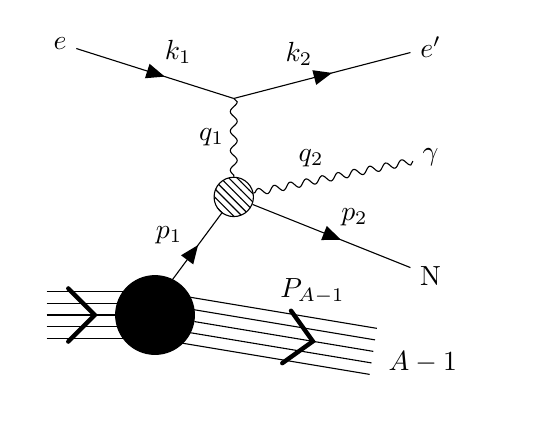
\begin{tikzpicture}
      \begin{feynman}
         \vertex                                            (n0) {};
         \vertex[large, blob, fill=black,right=1.5cm of n0] (n1) {};

         % incoming A nucleons
         \vertex[above = 0.15cm of n0]  (n01){~};
         \vertex[above = 0.30cm of n0]  (n02){~};
         \vertex[above = 0.45cm of n0]  (n03){~};
         \vertex[below = 0.15cm of n0]  (n04){~};
         \vertex[below = 0.30cm of n0]  (n05){~};
         \vertex[below = 0.45cm of n0]  (n06){~};

         \vertex[above = 0.15cm of n1]  (n11){~};
         \vertex[above = 0.30cm of n1]  (n12){~};
         \vertex[above = 0.45cm of n1]  (n13){~};
         \vertex[below = 0.15cm of n1]  (n14){~};
         \vertex[below = 0.30cm of n1]  (n15){~};
         \vertex[below = 0.45cm of n1]  (n16){~};

         \vertex[below right=0.5cm and 3.0cm of n1]            (n2) {};
         %\vertex[label={[label distance=0.2cm]-130:label},blob, fill=black, 

         \vertex[below right=0.5cm and 3.0cm of n11]  (n21) {};
         \vertex[below right=0.5cm and 3.0cm of n12]  (n22) {};
         \vertex[below right=0.5cm and 3.0cm of n13]  (n23) {};
         \vertex[below right=0.5cm and 3.0cm of n14]  (n24) {};
         \vertex[below right=0.5cm and 3.0cm of n15]  (n25) {};
         \vertex[below right=0.5cm and 3.0cm of n16]  (n26) {};

         \vertex[below right=0.5cm and 1.5cm of n2]      (n3) {};

         %dvcs vertex
         \vertex[small, blob, above right=1.5cm and 1.0cm of n1] (a0) {};

         % e,e'gamma vertex 
         \vertex[above=1.25cm of a0]                  (q0);

         \vertex[below right=1.0cm and 2.5cm of a0]  (a1) {N};
         \vertex[above=1.5cm of a1]                  (q1){\(\gamma\)};

         % electron
         \vertex[above left=0.5cm and 2.0cm of q0]  (e0) {\(e\)};
         \vertex[above=1.4 of q1]   (e1) {\(e^{\prime}\)};

         \diagram*{
            (e0) -- [fermion, edge label=\(k_1\)] (q0) -- [fermion, edge 
            label=\(k_2\)] (e1),
            (n11) -- [fermion, edge label=\(p_1\)] (a0) -- [fermion, edge label 
            = \(p_2\)] (a1),
            (a0) -- [photon, edge label = \(q_1\)] (q0),
            (a0) -- [photon, edge label = \(q_2\)] (q1),
            (n01) --  (n11)  --  (n21),
            (n02) --  (n12)  --  (n22),
            %(n03) --  (n13) --  (n23),
            (n04) --  (n14)  --  (n24),
            (n05) --  (n15)  --  (n25),
            %(n06) --  (n16) ,
            (n0) -- [plain,arrow size=6pt, postaction={decorate}, 
            decoration={markings, mark=at position 0.75 with 
         {\arrow[scale=4]{angle 90}}}] (n1) --
         [plain,arrow size=6pt, postaction={decorate}, decoration={markings, 
         mark=at position 0.65 with {\arrow[scale=4]{angle 90}}}] (n2),
         };

         \draw[fill,white,rotate=-9] ($(n2.west)-(0.10cm,0.35cm)$) rectangle 
         ($(n2.west)+(0.10cm,0.35cm)$);
         \vertex[below right=0.1cm and 0.4cm of n2]      (pminus1) {$A-1$};
         \vertex[above left=0.8cm and 1.0cm of n2]      (pm1label) {$P_{A-1}$};

         %% alert detection
         %\draw [decoration={brace,amplitude=7pt}, decorate]
         %($(n2.north east)+(1.0cm,0.3cm)$) -- ++(-0.4cm,-1.4cm);
         %\node[] at ($(n2.east)+(1.7cm,-0.4cm)$) {ALERT};

         %% CLAS12 detection
         %\draw [decoration={brace,amplitude=7pt}, decorate]
         %($(e1.east)+(0.0cm,0.2cm)$) -- ++(-0.0cm,-2.8cm);
         %\node[] at ($(e1.east)+(1.0cm,-1.2cm)$) {CLAS12};

      \end{feynman}
   \end{tikzpicture}
\end{center}
\caption{F}
\end{figure}

\begin{figure}
\begin{center}
   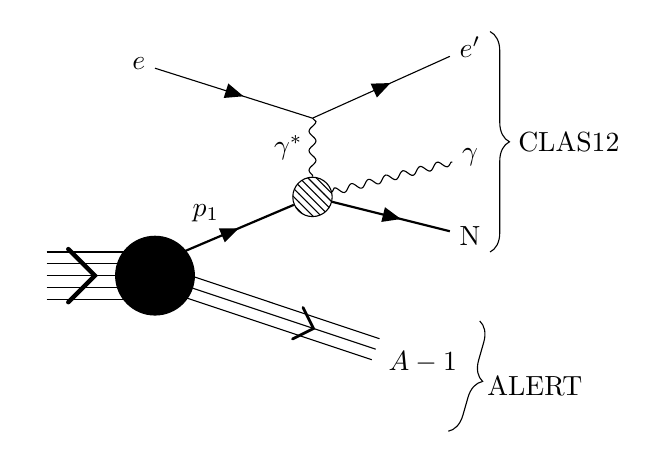
\begin{tikzpicture}
      \begin{feynman}
         \vertex                                            (n0) {};
         \vertex[large, blob, fill=black,right=1.5cm of n0] (n1) {};

         % incoming A nucleons
         \vertex[above = 0.15cm of n0]  (n01){~};
         \vertex[above = 0.30cm of n0]  (n02){~};
         \vertex[above = 0.45cm of n0]  (n03){~};
         \vertex[below = 0.15cm of n0]  (n04){~};
         \vertex[below = 0.30cm of n0]  (n05){~};
         \vertex[below = 0.45cm of n0]  (n06){~};

         \vertex[above = 0.15cm of n1]  (n11){~};
         \vertex[above = 0.30cm of n1]  (n12){~};
         \vertex[above = 0.45cm of n1]  (n13){~};
         \vertex[below = 0.15cm of n1]  (n14){~};
         \vertex[below = 0.30cm of n1]  (n15){~};
         \vertex[below = 0.45cm of n1]  (n16){~};

         \vertex[below right=1.0cm and 3.0cm of n1]            (n2) {};
         %\vertex[label={[label distance=0.2cm]-130:label},blob, fill=black, 

         \vertex[below right=1.0cm and 3.0cm of n11]  (n21) {};
         \vertex[below right=1.0cm and 3.0cm of n12]  (n22) {};
         \vertex[below right=1.0cm and 3.0cm of n13]  (n23) {};
         \vertex[below right=1.0cm and 3.0cm of n14]  (n24) {};
         \vertex[below right=1.0cm and 3.0cm of n15]  (n25) {};
         \vertex[below right=1.0cm and 3.0cm of n16]  (n26) {};

         \vertex[below right=0.5cm and 1.5cm of n2]      (n3) {};

         %dvcs vertex
         \vertex[small, blob, above right=1.0cm and 2.0cm of n1] (a0) {};

         % e,e'gamma vertex 
         \vertex[above=1.0cm of a0]                  (q0);

         \vertex[below right=0.5cm and 2.0cm of a0]  (a1) {N};
         \vertex[above=1.0cm of a1]                  (q1){\(\gamma\)};

         % fsi
         \node[left=1.15cm of a1]                 (a10);

         % electron
         \vertex[above left=0.5cm and 2.0cm of q0]  (e0) {\(e\)};
         \vertex[above=1.4 of q1]   (e1) {\(e^{\prime}\)};

         \diagram*{
            (e0) -- [fermion] (q0) -- [fermion] (e1),
            (n11) -- [thick,fermion, edge label=\(p_1\)] (a0),
            (a0) -- [thick, fermion] (a1),
            (a0) -- [photon, edge label = \(\gamma^{*}\)] (q0),
            (q1) -- [photon] (a0),
            (n01) --  (n11)  --  (n21),
            (n02) --  (n12),  %--  (n22),
            %(n03) --  (n13) --  (n23),
            (n04) --  (n14)  --  (n24),
            (n05) --  (n15),%  --  (n25),
            %(n06) --  (n16) ,
            (n0) -- [plain,arrow size=6pt, postaction={decorate}, 
            decoration={markings, mark=at position 0.75 with 
         {\arrow[scale=4]{angle 90}}}](n1)
         -- [plain,arrow size=6pt, postaction={decorate}, decoration={markings, 
         mark=at position 0.65 with {\arrow[scale=2.5]{angle 90}}}](n2),
         %-- [fermion, edge label = \(p_{A-1}\)] (n3),
         };

         % alert detection
         \draw [decoration={brace,amplitude=7pt}, decorate]
         ($(n2.north east)+(1.0cm,0.3cm)$) -- ++(-0.4cm,-1.4cm);
         \node[] at ($(n2.east)+(1.7cm,-0.4cm)$) {ALERT};

         % CLAS12 detection
         \draw [decoration={brace,amplitude=7pt}, decorate]
         ($(e1.east)+(0.0cm,0.2cm)$) -- ++(-0.0cm,-2.8cm);
         \node[] at ($(e1.east)+(1.0cm,-1.2cm)$) {CLAS12};

         \draw[fill,white,rotate=-20] ($(n2)-(0.20cm,0.3cm)$) rectangle 
         ($(n2)+(0.20cm,0.3cm)$);
         \vertex[below right=0.1cm and 0.4cm of n2]      (pminus1) {$A-1$};

      \end{feynman}
   \end{tikzpicture}
\end{center}
\caption{G}
\end{figure}

\begin{figure}
\begin{center}
   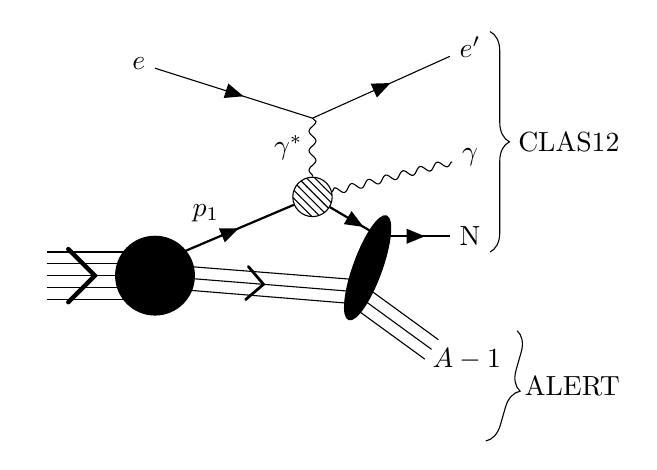
\begin{tikzpicture}
      \begin{feynman}
         \vertex                                            (n0) {};
         \vertex[large, blob, fill=black,right=1.5cm of n0] (n1) {};

         % incoming A nucleons
         \vertex[above = 0.15cm of n0]  (n01){~};
         \vertex[above = 0.30cm of n0]  (n02){~};
         \vertex[above = 0.45cm of n0]  (n03){~};
         \vertex[below = 0.15cm of n0]  (n04){~};
         \vertex[below = 0.30cm of n0]  (n05){~};
         \vertex[below = 0.45cm of n0]  (n06){~};

         \vertex[above = 0.15cm of n1]  (n11){~};
         \vertex[above = 0.30cm of n1]  (n12){~};
         \vertex[above = 0.45cm of n1]  (n13){~};
         \vertex[below = 0.15cm of n1]  (n14){~};
         \vertex[below = 0.30cm of n1]  (n15){~};
         \vertex[below = 0.45cm of n1]  (n16){~};

         %\vertex[label={[label distance=0.2cm]-130:label},blob, fill=black, 


         \vertex[below right=0.2cm and 2.5cm of n1]   (n2)  ;
         \vertex[below right=0.2cm and 2.55cm of n11]  (n21) ;
         \vertex[below right=0.2cm and 2.45cm of n14]  (n24) ;

         \vertex[below right=0.8cm and 1.1cm of n2]   (n3)  ;
         \vertex[below right=0.8cm and 1.1cm of n21]  (n31) ;
         \vertex[below right=0.8cm and 1.1cm of n24]  (n34) ;


         %dvcs vertex
         \vertex[small, blob, above right=1.0cm and 2.0cm of n1] (a0) {};


         % e,e'gamma vertex 
         \vertex[above=1.0cm of a0]                  (q0);

         \vertex[below right=0.5cm and 2.0cm of a0]  (a1) {N};
         \vertex[above=1.0cm of a1]                  (q1){\(\gamma\)};

         % fsi
         \vertex[above right=0.1cm and 2.7cm of n1] (fsi);
         \vertex[left=1.15cm of a1]              (a10);

         % electron
         \vertex[above left=0.5cm and 2.0cm of q0]  (e0) {\(e\)};
         \vertex[above=1.4 of q1]   (e1) {\(e^{\prime}\)};

         \diagram*{
            (e0) -- [fermion] (q0) -- [fermion] (e1),
            (n11) -- [thick,fermion, edge label=\(p_1\)] (a0),
            (a0) -- [thick, fermion] (a10) -- [thick, fermion] (a1),
            (a0) -- [photon, edge label = \(\gamma^{*}\)] (q0),
            (q1) -- [photon] (a0),
            (n01) --  (n11)  --  (n21) -- (n31),
            (n02) --  (n12),  %--  (n22),
            %(n03) --  (n13) --  (n23),
            (n04) --  (n14)  --  (n24) -- (n34),
            (n05) --  (n15),%  --  (n25),
            %(n06) --  (n16) ,
            (n0) -- [plain,arrow size=6pt, postaction={decorate}, 
            decoration={markings, mark=at position 0.75 with 
         {\arrow[scale=4]{angle 90}}}](n1)
         -- [plain,arrow size=6pt, postaction={decorate}, decoration={markings, 
         mark=at position 0.45 with {\arrow[scale=2.5]{angle 
   90}}}](n2)--[plain](n3),
         %-- [fermion, edge label = \(p_{A-1}\)] (n3),
         };

         % alert detection
         \draw [decoration={brace,amplitude=7pt}, decorate]
         ($(n3.north east)+(1.0cm,0.3cm)$) -- ++(-0.4cm,-1.4cm);
         \node[] at ($(n3.east)+(1.7cm,-0.4cm)$) {ALERT};


         % CLAS12 detection
         \draw [decoration={brace,amplitude=7pt}, decorate]
         ($(e1.east)+(0.0cm,0.2cm)$) -- ++(-0.0cm,-2.8cm);
         \node[] at ($(e1.east)+(1.0cm,-1.2cm)$) {CLAS12};

         \draw[fill,black,rotate=-20] (fsi) ellipse (0.18cm and 0.7cm);

         \draw[fill,white,rotate=-35] ($(n3)-(0.10cm,0.3cm)$) rectangle 
         ($(n3)+(0.10cm,0.3cm)$);
         \vertex[below right=-0.2cm and -0.2cm of n3]    (pminus1) {$A-1$};

      \end{feynman}
   \end{tikzpicture}
\end{center}
\caption{H}
\end{figure}


\begin{figure}
\begin{center}
   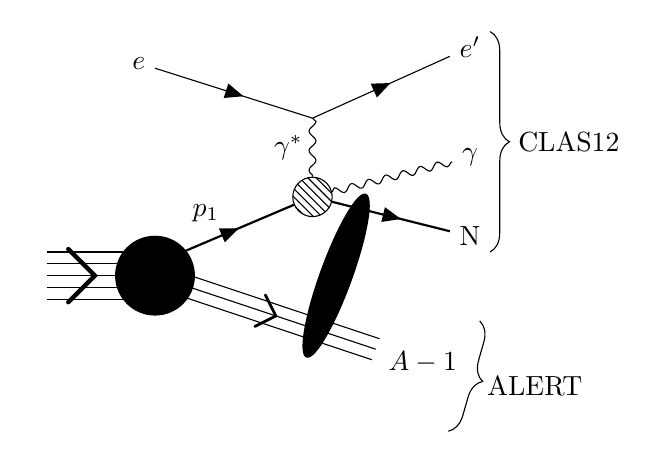
\begin{tikzpicture}
      \begin{feynman}
         \vertex                                            (n0) {};
         \vertex[large, blob, fill=black,right=1.5cm of n0] (n1) {};

         % incoming A nucleons
         \vertex[above = 0.15cm of n0]  (n01){~};
         \vertex[above = 0.30cm of n0]  (n02){~};
         \vertex[above = 0.45cm of n0]  (n03){~};
         \vertex[below = 0.15cm of n0]  (n04){~};
         \vertex[below = 0.30cm of n0]  (n05){~};
         \vertex[below = 0.45cm of n0]  (n06){~};

         \vertex[above = 0.15cm of n1]  (n11){~};
         \vertex[above = 0.30cm of n1]  (n12){~};
         \vertex[above = 0.45cm of n1]  (n13){~};
         \vertex[below = 0.15cm of n1]  (n14){~};
         \vertex[below = 0.30cm of n1]  (n15){~};
         \vertex[below = 0.45cm of n1]  (n16){~};

         \vertex[below right=1.0cm and 3.0cm of n1]            (n2) {};
         %\vertex[label={[label distance=0.2cm]-130:label},blob, fill=black, 

         \vertex[right=2.3cm of n1]            (fsi) {};

         \vertex[below right=1.0cm and 3.0cm of n11]  (n21) {};
         \vertex[below right=1.0cm and 3.0cm of n12]  (n22) {};
         \vertex[below right=1.0cm and 3.0cm of n13]  (n23) {};
         \vertex[below right=1.0cm and 3.0cm of n14]  (n24) {};
         \vertex[below right=1.0cm and 3.0cm of n15]  (n25) {};
         \vertex[below right=1.0cm and 3.0cm of n16]  (n26) {};

         \vertex[below right=0.5cm and 1.5cm of n2]      (n3) {};

         %dvcs vertex
         \vertex[small, blob, above right=1.0cm and 2.0cm of n1] (a0) {};

         % e,e'gamma vertex 
         \vertex[above=1.0cm of a0]                  (q0);

         \vertex[below right=0.5cm and 2.0cm of a0]  (a1) {N};
         \vertex[above=1.0cm of a1]                  (q1){\(\gamma\)};

         % electron
         \vertex[above left=0.5cm and 2.0cm of q0]  (e0) {\(e\)};
         \vertex[above=1.4 of q1]   (e1) {\(e^{\prime}\)};

         \diagram*{
            (e0) -- [fermion] (q0) -- [fermion] (e1),
            (n11) -- [thick,fermion, edge label=\(p_1\)] (a0) -- [thick, 
            fermion] (a1),
            (a0) -- [photon, edge label = \(\gamma^{*}\)] (q0),
            (q1) -- [photon] (a0),
            (n01) --  (n11)  --  (n21),
            (n02) --  (n12),  %--  (n22),
            %(n03) --  (n13) --  (n23),
            (n04) --  (n14)  --  (n24),
            (n05) --  (n15),%  --  (n25),
            %(n06) --  (n16) ,
            (n0) -- [plain,arrow size=6pt, postaction={decorate}, 
            decoration={markings, mark=at position 0.75 with 
         {\arrow[scale=4]{angle 90}}}](n1)
         -- [plain,arrow size=6pt, postaction={decorate}, decoration={markings, 
         mark=at position 0.45 with {\arrow[scale=2.5]{angle 90}}}](n2),
         %-- [fermion, edge label = \(p_{A-1}\)] (n3),
         };

         % alert detection
         \draw [decoration={brace,amplitude=7pt}, decorate]
         ($(n2.north east)+(1.0cm,0.3cm)$) -- ++(-0.4cm,-1.4cm);
         \node[] at ($(n2.east)+(1.7cm,-0.4cm)$) {ALERT};

         % CLAS12 detection
         \draw [decoration={brace,amplitude=7pt}, decorate]
         ($(e1.east)+(0.0cm,0.2cm)$) -- ++(-0.0cm,-2.8cm);
         \node[] at ($(e1.east)+(1.0cm,-1.2cm)$) {CLAS12};

         \draw[fill,black,rotate=-20] (fsi) ellipse (0.20cm and 1.1cm);

         \draw[fill,white,rotate=-20] ($(n2)-(0.20cm,0.3cm)$) rectangle 
         ($(n2)+(0.20cm,0.3cm)$);
         \vertex[below right=0.1cm and 0.4cm of n2]      (pminus1) {$A-1$};

      \end{feynman}
   \end{tikzpicture}
\end{center}
\caption{I}
\end{figure}

\begin{figure}
\begin{center}
   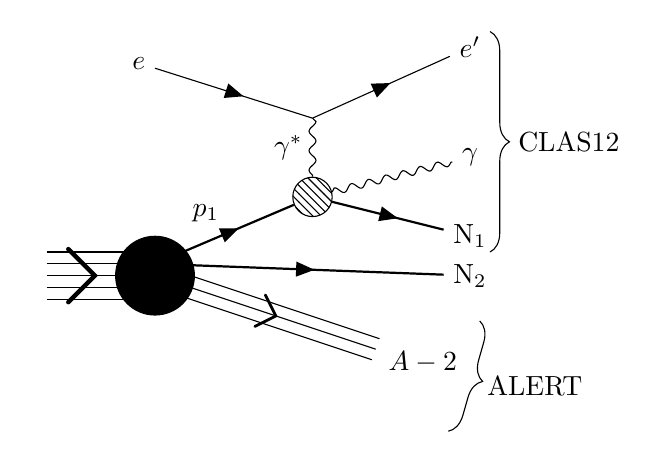
\begin{tikzpicture}
      \begin{feynman}
         \vertex                                            (n0) {};
         \vertex[large, blob, fill=black,right=1.5cm of n0] (n1) {};

         % incoming A nucleons
         \vertex[above = 0.15cm of n0]  (n01){~};
         \vertex[above = 0.30cm of n0]  (n02){~};
         \vertex[above = 0.45cm of n0]  (n03){~};
         \vertex[below = 0.15cm of n0]  (n04){~};
         \vertex[below = 0.30cm of n0]  (n05){~};
         \vertex[below = 0.45cm of n0]  (n06){~};

         \vertex[above = 0.15cm of n1]  (n11){~};
         \vertex[above = 0.30cm of n1]  (n12){~};
         \vertex[above = 0.45cm of n1]  (n13){~};
         \vertex[below = 0.15cm of n1]  (n14){~};
         \vertex[below = 0.30cm of n1]  (n15){~};
         \vertex[below = 0.45cm of n1]  (n16){~};

         \vertex[below right=1.0cm and 3.0cm of n1]            (n2) {};
         %\vertex[label={[label distance=0.2cm]-130:label},blob, fill=black, 

         \vertex[right=2.3cm of n1]            (fsi) {};

         \vertex[below right=1.0cm and 3.0cm of n11]  (n21) {};
         \vertex[below right=1.0cm and 3.0cm of n12]  (n22) {};
         \vertex[below right=1.0cm and 3.0cm of n13]  (n23) {};
         \vertex[below right=1.0cm and 3.0cm of n14]  (n24) {};
         \vertex[below right=1.0cm and 3.0cm of n15]  (n25) {};
         \vertex[below right=1.0cm and 3.0cm of n16]  (n26) {};

         \vertex[below right=0.5cm and 1.5cm of n2]      (n3) {};

         %dvcs vertex
         \vertex[small, blob, above right=1.0cm and 2.0cm of n1] (a0) {};

         % e,e'gamma vertex 
         \vertex[above=1.0cm of a0]                  (q0);

         \vertex[below right=0.5cm and 2.0cm of a0]  (a1) {N$_1$};
         \vertex[above=1.0cm of a1]                  (q1){\(\gamma\)};
         \vertex[below=0.5cm of a1]  (a2) {N$_2$};

         % electron
         \vertex[above left=0.5cm and 2.0cm of q0]  (e0) {\(e\)};
         \vertex[above=1.4 of q1]   (e1) {\(e^{\prime}\)};

         \diagram*{
            (e0) -- [fermion] (q0) -- [fermion] (e1),
            (n11) -- [thick,fermion, edge label=\(p_1\)] (a0) 
            -- [thick, fermion] (a1),
            (n11) -- [thick,fermion] (a2),
            (a0) -- [photon, edge label = \(\gamma^{*}\)] (q0),
            (q1) -- [photon] (a0),
            (n01) --  (n11)  --  (n21),
            (n02) --  (n12),  %--  (n22),
            %(n03) --  (n13) --  (n23),
            (n04) --  (n14)  --  (n24),
            (n05) --  (n15),%  --  (n25),
            %(n06) --  (n16) ,
            (n0) -- [plain,arrow size=6pt, postaction={decorate}, 
            decoration={markings, mark=at position 0.75 with 
         {\arrow[scale=4]{angle 90}}}](n1)
         -- [plain,arrow size=6pt, postaction={decorate}, decoration={markings, 
         mark=at position 0.45 with {\arrow[scale=2.5]{angle 90}}}](n2),
         %-- [fermion, edge label = \(p_{A-1}\)] (n3),
         };

         % alert detection
         \draw [decoration={brace,amplitude=7pt}, decorate]
         ($(n2.north east)+(1.0cm,0.3cm)$) -- ++(-0.4cm,-1.4cm);
         \node[] at ($(n2.east)+(1.7cm,-0.4cm)$) {ALERT};

         % CLAS12 detection
         \draw [decoration={brace,amplitude=7pt}, decorate]
         ($(e1.east)+(0.0cm,0.2cm)$) -- ++(-0.0cm,-2.8cm);
         \node[] at ($(e1.east)+(1.0cm,-1.2cm)$) {CLAS12};

         %\draw[fill,black,rotate=-20] (fsi) ellipse (0.20cm and 1.1cm);

         \draw[fill,white,rotate=-20] ($(n2)-(0.20cm,0.3cm)$) rectangle 
         ($(n2)+(0.20cm,0.3cm)$);
         \vertex[below right=0.1cm and 0.4cm of n2]      (pminus1) {$A-2$};

      \end{feynman}
   \end{tikzpicture}
\end{center}
\caption{J}
\end{figure}

\begin{figure}
\begin{center}
   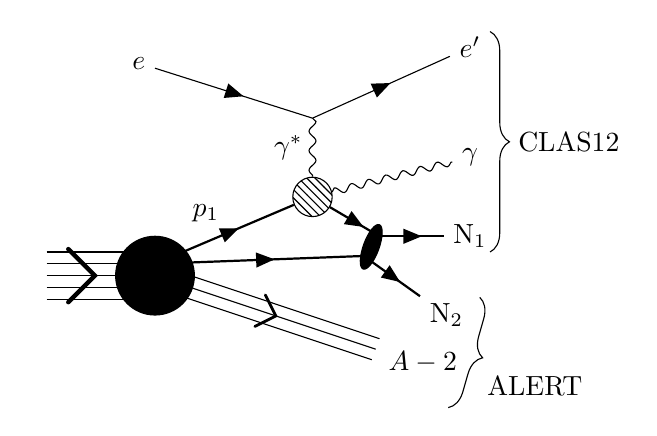
\begin{tikzpicture}
      \begin{feynman}
         \vertex                                            (n0) {};
         \vertex[large, blob, fill=black,right=1.5cm of n0] (n1) {};

         % incoming A nucleons
         \vertex[above = 0.15cm of n0]  (n01){~};
         \vertex[above = 0.30cm of n0]  (n02){~};
         \vertex[above = 0.45cm of n0]  (n03){~};
         \vertex[below = 0.15cm of n0]  (n04){~};
         \vertex[below = 0.30cm of n0]  (n05){~};
         \vertex[below = 0.45cm of n0]  (n06){~};

         \vertex[above = 0.15cm of n1]  (n11){~};
         \vertex[above = 0.30cm of n1]  (n12){~};
         \vertex[above = 0.45cm of n1]  (n13){~};
         \vertex[below = 0.15cm of n1]  (n14){~};
         \vertex[below = 0.30cm of n1]  (n15){~};
         \vertex[below = 0.45cm of n1]  (n16){~};

         \vertex[below right=1.0cm and 3.0cm of n1]            (n2) {};
         %\vertex[label={[label distance=0.2cm]-130:label},blob, fill=black, 


         \vertex[below right=1.0cm and 3.0cm of n11]  (n21) {};
         \vertex[below right=1.0cm and 3.0cm of n12]  (n22) {};
         \vertex[below right=1.0cm and 3.0cm of n13]  (n23) {};
         \vertex[below right=1.0cm and 3.0cm of n14]  (n24) {};
         \vertex[below right=1.0cm and 3.0cm of n15]  (n25) {};
         \vertex[below right=1.0cm and 3.0cm of n16]  (n26) {};

         \vertex[below right=0.5cm and 1.5cm of n2]      (n3) {};

         %dvcs vertex
         \vertex[small, blob, above right=1.0cm and 2.0cm of n1] (a0) {};

         % e,e'gamma vertex 
         \vertex[above=1.0cm of a0]                  (q0);

         \vertex[below right=0.5cm and 2.0cm of a0]  (a1) {N$_1$};
         \vertex[below left=1.0cm and 0.3cm of a1]   (a2) {N$_2$};

         \vertex[above=1.0cm of a1]                  (q1){\(\gamma\)};

         % fsi
         \vertex[left=1.15cm of a1]                 (a10);
         \vertex[below left=0.25cm and 0.2 of a10]    (a20);

         % electron
         \vertex[above left=0.5cm and 2.0cm of q0]  (e0) {\(e\)};
         \vertex[above=1.4 of q1]   (e1) {\(e^{\prime}\)};

         \diagram*{
            (e0) -- [fermion] (q0) -- [fermion] (e1),
            (n11) -- [thick,fermion,edge label=\(p_1\)] (a0),
            (a0) -- [thick,fermion] (a10) -- [thick, fermion] (a1),
            (n11) -- [thick,fermion] (a20)-- [thick,fermion] (a2),
            (a0) -- [photon, edge label = \(\gamma^{*}\)] (q0),
            (q1) -- [photon] (a0),
            (n01) --  (n11)  --  (n21),
            (n02) --  (n12),  %--  (n22),
            %(n03) --  (n13) --  (n23),
            (n04) --  (n14)  --  (n24),
            (n05) --  (n15),%  --  (n25),
            %(n06) --  (n16) ,
            (n0) -- [plain,arrow size=6pt, postaction={decorate}, 
            decoration={markings, mark=at position 0.75 with 
         {\arrow[scale=4]{angle 90}}}](n1)
         -- [plain,arrow size=6pt, postaction={decorate}, decoration={markings, 
         mark=at position 0.45 with {\arrow[scale=2.5]{angle 90}}}](n2),
         %-- [fermion, edge label = \(p_{A-1}\)] (n3),
         };

         % alert detection
         \draw [decoration={brace,amplitude=7pt}, decorate]
         ($(n2.north east)+(1.0cm,0.6cm)$) -- ++(-0.4cm,-1.4cm);
         \node[] at ($(n2.east)+(1.7cm,-0.4cm)$) {ALERT};

         % CLAS12 detection
         \draw [decoration={brace,amplitude=7pt}, decorate]
         ($(e1.east)+(0.0cm,0.2cm)$) -- ++(-0.0cm,-2.8cm);
         \node[] at ($(e1.east)+(1.0cm,-1.2cm)$) {CLAS12};

         % FSI ellipse
         \node[below left=0.01cm and -0.02cm of a10]            (fsi) {};
         \draw[fill,black,rotate=-20] (fsi) ellipse (0.10cm and 0.3cm);

         \draw[fill,white,rotate=-20] ($(n2)-(0.20cm,0.3cm)$) rectangle 
         ($(n2)+(0.20cm,0.3cm)$);
         \vertex[below right=0.1cm and 0.4cm of n2]      (pminus1) {$A-2$};

      \end{feynman}
   \end{tikzpicture}
\end{center}
\caption{K}
\end{figure}

\begin{figure}
\begin{center}
   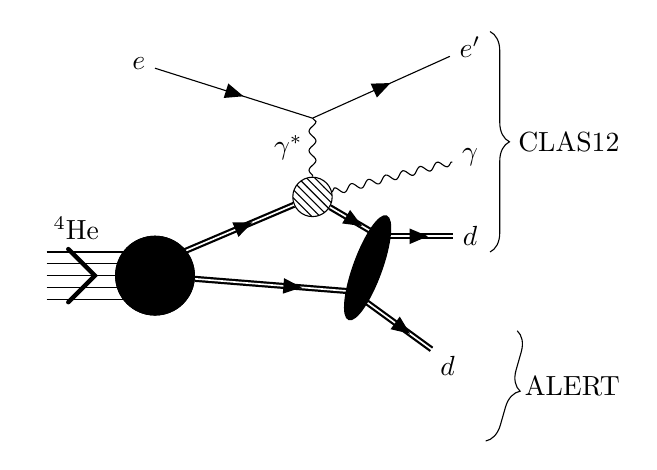
\begin{tikzpicture}[
         deuteron/.style = {double,thick,arrow size=0.5pt, 
      postaction={decorate}, decoration={markings, mark=at position 0.70 with 
{\arrow[scale=0.6]{triangle 45}}}}]

      \begin{feynman}
         \vertex                                            (n0) {};
         \vertex[large, blob, fill=black,right=1.5cm of n0] (n1) {};

         \vertex[above right=0.6cm and 0.5 of n0]   (Ain) {$^4$He};

         % incoming A nucleons
         \vertex[above = 0.15cm of n0]  (n01){~};
         \vertex[above = 0.30cm of n0]  (n02){~};
         \vertex[above = 0.45cm of n0]  (n03){~};
         \vertex[below = 0.15cm of n0]  (n04){~};
         \vertex[below = 0.30cm of n0]  (n05){~};
         \vertex[below = 0.45cm of n0]  (n06){~};

         \vertex[above = 0.15cm of n1]  (n11){~};
         \vertex[above = 0.30cm of n1]  (n12){~};
         \vertex[above = 0.45cm of n1]  (n13){~};
         \vertex[below = 0.15cm of n1]  (n14){~};
         \vertex[below = 0.30cm of n1]  (n15){~};
         \vertex[below = 0.45cm of n1]  (n16){~};

         %\vertex[label={[label distance=0.2cm]-130:label},blob, fill=black, 


         \vertex[below right=0.2cm and 2.5cm of n1]   (n2)  ;
         \vertex[below right=0.2cm and 2.55cm of n11]  (n21) ;
         \vertex[below right=0.2cm and 2.45cm of n14]  (n24) ;

         \vertex[below right=0.8cm and 1.1cm of n2]   (n3)  ;
         \vertex[below right=0.8cm and 1.1cm of n21]  (n31) ;
         \vertex[below right=0.8cm and 1.1cm of n24]  (n34) ;


         %dvcs vertex
         \vertex[small, blob, above right=1.0cm and 2.0cm of n1] (a0) {};


         % e,e'gamma vertex 
         \vertex[above=1.0cm of a0]                  (q0);

         \vertex[below right=0.5cm and 2.0cm of a0]  (a1) {$d$};
         \vertex[above=1.0cm of a1]                  (q1){\(\gamma\)};

         % fsi
         \vertex[above right=0.1cm and 2.7cm of n1] (fsi);
         \vertex[left=1.15cm of a1]              (a10);

         % electron
         \vertex[above left=0.5cm and 2.0cm of q0]  (e0) {\(e\)};
         \vertex[above=1.4 of q1]   (e1) {\(e^{\prime}\)};

         \diagram*{
            (e0) -- [fermion] (q0) -- [fermion] (e1),
            (n11) -- [deuteron] (a0),
            (a0) -- [deuteron] (a10) -- [deuteron] (a1),
            (a0) -- [photon, edge label = \(\gamma^{*}\)] (q0),
            (q1) -- [photon] (a0),
            (n01) --  (n11),%  --  (n21) -- (n31),
            (n02) --  (n12),  %--  (n22),
            %(n03) --  (n13) --  (n23),
            (n04) --  (n14),%  --  (n24) -- (n34),
            (n05) --  (n15),%  --  (n25),
            %(n06) --  (n16) ,
            (n0) -- [plain,arrow size=6pt, postaction={decorate}, 
            decoration={markings, mark=at position 0.75 with 
         {\arrow[scale=4]{angle 90}}}](n1)
         -- [deuteron](n2)--[deuteron](n3),
         %-- [fermion, edge label = \(p_{A-1}\)] (n3),
         };

         %fill in the blob again
         \vertex[large, blob, fill=black,right=1.5cm of n0] {};

         % alert detection
         \draw [decoration={brace,amplitude=7pt}, decorate]
         ($(n3.north east)+(1.0cm,0.3cm)$) -- ++(-0.4cm,-1.4cm);
         \node[] at ($(n3.east)+(1.7cm,-0.4cm)$) {ALERT};

         % CLAS12 detection
         \draw [decoration={brace,amplitude=7pt}, decorate]
         ($(e1.east)+(0.0cm,0.2cm)$) -- ++(-0.0cm,-2.8cm);
         \node[] at ($(e1.east)+(1.0cm,-1.2cm)$) {CLAS12};

         \draw[fill,black,rotate=-20] (fsi) ellipse (0.18cm and 0.7cm);

         \draw[fill,white,rotate=-35] ($(n3)-(0.10cm,0.3cm)$) rectangle 
         ($(n3)+(0.10cm,0.3cm)$);
         \vertex[below right=-0.1cm and -0.1cm of n3]    (pminus1) {$d$};

      \end{feynman}
   \end{tikzpicture}
\end{center}
\caption{L}
\end{figure}

\begin{figure}
\begin{center}
   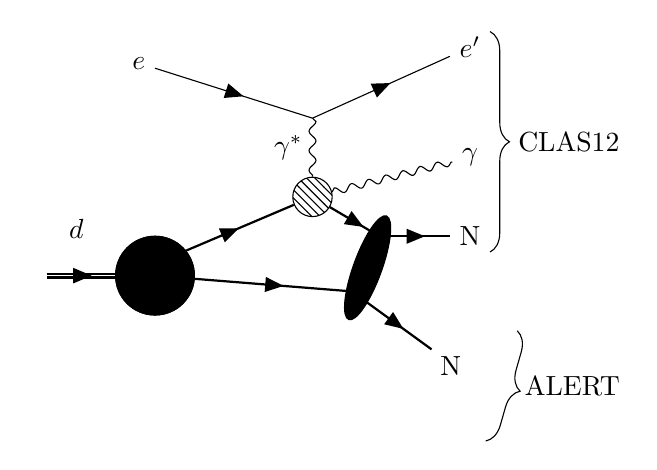
\begin{tikzpicture}[
         nucleon/.style = {thick,fermion},
         deuteron/.style = {double,thick,arrow size=0.5pt, 
         postaction={decorate}, decoration={markings, mark=at position 0.70 
      with {\arrow[scale=0.6]{triangle 45}}}}
]

      \begin{feynman}
         \vertex                                            (n0) {};
         \vertex[large, blob, fill=black,right=1.5cm of n0] (n1) {};

         \vertex[above right=0.6cm and 0.5 of n0]   (Ain) {$d$};

         % incoming A nucleons
         \vertex[above = 0.15cm of n0]  (n01){~};
         \vertex[above = 0.30cm of n0]  (n02){~};
         \vertex[above = 0.45cm of n0]  (n03){~};
         \vertex[below = 0.15cm of n0]  (n04){~};
         \vertex[below = 0.30cm of n0]  (n05){~};
         \vertex[below = 0.45cm of n0]  (n06){~};

         \vertex[above = 0.15cm of n1]  (n11){~};
         \vertex[above = 0.30cm of n1]  (n12){~};
         \vertex[above = 0.45cm of n1]  (n13){~};
         \vertex[below = 0.15cm of n1]  (n14){~};
         \vertex[below = 0.30cm of n1]  (n15){~};
         \vertex[below = 0.45cm of n1]  (n16){~};

         %\vertex[label={[label distance=0.2cm]-130:label},blob, fill=black, 


         \vertex[below right=0.2cm and 2.5cm of n1]   (n2)  ;
         \vertex[below right=0.2cm and 2.55cm of n11]  (n21) ;
         \vertex[below right=0.2cm and 2.45cm of n14]  (n24) ;

         \vertex[below right=0.8cm and 1.1cm of n2]   (n3)  ;
         \vertex[below right=0.8cm and 1.1cm of n21]  (n31) ;
         \vertex[below right=0.8cm and 1.1cm of n24]  (n34) ;


         %dvcs vertex
         \vertex[small, blob, above right=1.0cm and 2.0cm of n1] (a0) {};


         % e,e'gamma vertex 
         \vertex[above=1.0cm of a0]                  (q0);

         \vertex[below right=0.5cm and 2.0cm of a0]  (a1) {N};
         \vertex[above=1.0cm of a1]                  (q1){\(\gamma\)};

         % fsi
         \vertex[above right=0.1cm and 2.7cm of n1] (fsi);
         \vertex[left=1.15cm of a1]              (a10);

         % electron
         \vertex[above left=0.5cm and 2.0cm of q0]  (e0) {\(e\)};
         \vertex[above=1.4 of q1]   (e1) {\(e^{\prime}\)};

         \diagram*{
            (e0) -- [fermion] (q0) -- [fermion] (e1),
            (n11) -- [nucleon] (a0),
            (a0) -- [nucleon] (a10) -- [nucleon] (a1),
            (a0) -- [photon, edge label = \(\gamma^{*}\)] (q0),
            (q1) -- [photon] (a0),
            %(n01) --  (n11),%  --  (n21) -- (n31),
            %(n02) --  (n12),  %--  (n22),
            %(n03) --  (n13) --  (n23),
            %(n04) --  (n14),%  --  (n24) -- (n34),
            %(n05) --  (n15),%  --  (n25),
            %(n06) --  (n16) ,
            (n0) -- [deuteron](n1) -- [nucleon](n2)--[nucleon](n3),
         %-- [fermion, edge label = \(p_{A-1}\)] (n3),
         };

         %fill in the blob again
         \vertex[large, blob, fill=black,right=1.5cm of n0] {};

         % alert detection
         \draw [decoration={brace,amplitude=7pt}, decorate]
         ($(n3.north east)+(1.0cm,0.3cm)$) -- ++(-0.4cm,-1.4cm);
         \node[] at ($(n3.east)+(1.7cm,-0.4cm)$) {ALERT};

         % CLAS12 detection
         \draw [decoration={brace,amplitude=7pt}, decorate]
         ($(e1.east)+(0.0cm,0.2cm)$) -- ++(-0.0cm,-2.8cm);
         \node[] at ($(e1.east)+(1.0cm,-1.2cm)$) {CLAS12};

         \draw[fill,black,rotate=-20] (fsi) ellipse (0.18cm and 0.7cm);

         \draw[fill,white,rotate=-35] ($(n3)-(0.10cm,0.3cm)$) rectangle 
         ($(n3)+(0.10cm,0.3cm)$);
         \vertex[below right=-0.1cm and -0.1cm of n3]    (pminus1) {N};

      \end{feynman}
   \end{tikzpicture}
\end{center}
\caption{M}
\end{figure}



\begin{figure}
\begin{center}
   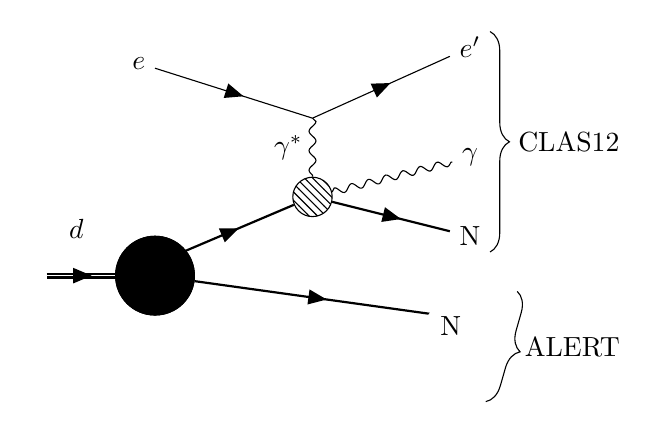
\begin{tikzpicture}[
         nucleon/.style = {thick,fermion},
         deuteron/.style = {double,thick,arrow size=0.5pt, 
         postaction={decorate}, decoration={markings, mark=at position 0.70 
      with {\arrow[scale=0.6]{triangle 45}}}}
]

      \begin{feynman}
         \vertex                                            (n0) {};
         \vertex[large, blob, fill=black,right=1.5cm of n0] (n1) {};

         \vertex[above right=0.6cm and 0.5 of n0]   (Ain) {$d$};

         % incoming A nucleons
         \vertex[above = 0.15cm of n0]  (n01){~};
         \vertex[above = 0.30cm of n0]  (n02){~};
         \vertex[above = 0.45cm of n0]  (n03){~};
         \vertex[below = 0.15cm of n0]  (n04){~};
         \vertex[below = 0.30cm of n0]  (n05){~};
         \vertex[below = 0.45cm of n0]  (n06){~};

         \vertex[above = 0.15cm of n1]  (n11){~};
         \vertex[above = 0.30cm of n1]  (n12){~};
         \vertex[above = 0.45cm of n1]  (n13){~};
         \vertex[below = 0.15cm of n1]  (n14){~};
         \vertex[below = 0.30cm of n1]  (n15){~};
         \vertex[below = 0.45cm of n1]  (n16){~};

         %\vertex[label={[label distance=0.2cm]-130:label},blob, fill=black, 


         \vertex[below right=0.2cm and 2.5cm of n1]   (n2)  ;
         \vertex[below right=0.2cm and 2.55cm of n11]  (n21) ;
         \vertex[below right=0.2cm and 2.45cm of n14]  (n24) ;

         \vertex[below right=0.3cm and 1.1cm of n2]   (n3)  ;
         \vertex[below right=0.8cm and 1.1cm of n21]  (n31) ;
         \vertex[below right=0.8cm and 1.1cm of n24]  (n34) ;


         %dvcs vertex
         \vertex[small, blob, above right=1.0cm and 2.0cm of n1] (a0) {};


         % e,e'gamma vertex 
         \vertex[above=1.0cm of a0]                  (q0);

         \vertex[below right=0.5cm and 2.0cm of a0]  (a1) {N};
         \vertex[above=1.0cm of a1]                  (q1){\(\gamma\)};

         % fsi
         \vertex[above right=0.1cm and 2.7cm of n1] (fsi);
         \vertex[left=1.15cm of a1]              (a10);

         % electron
         \vertex[above left=0.5cm and 2.0cm of q0]  (e0) {\(e\)};
         \vertex[above=1.4 of q1]   (e1) {\(e^{\prime}\)};

         \diagram*{
            (e0) -- [fermion] (q0) -- [fermion] (e1),
            (n11) -- [nucleon] (a0),
            (a0)  -- [nucleon] (a1),
            (a0) -- [photon, edge label = \(\gamma^{*}\)] (q0),
            (q1) -- [photon] (a0),
            %(n01) --  (n11),%  --  (n21) -- (n31),
            %(n02) --  (n12),  %--  (n22),
            %(n03) --  (n13) --  (n23),
            %(n04) --  (n14),%  --  (n24) -- (n34),
            %(n05) --  (n15),%  --  (n25),
            %(n06) --  (n16) ,
            (n0) -- [deuteron](n1) -- [nucleon](n3),
         %-- [fermion, edge label = \(p_{A-1}\)] (n3),
         };

         %fill in the blob again
         \vertex[large, blob, fill=black,right=1.5cm of n0] {};

         % alert detection
         \draw [decoration={brace,amplitude=7pt}, decorate]
         ($(n3.north east)+(1.0cm,0.3cm)$) -- ++(-0.4cm,-1.4cm);
         \node[] at ($(n3.east)+(1.7cm,-0.4cm)$) {ALERT};

         % CLAS12 detection
         \draw [decoration={brace,amplitude=7pt}, decorate]
         ($(e1.east)+(0.0cm,0.2cm)$) -- ++(-0.0cm,-2.8cm);
         \node[] at ($(e1.east)+(1.0cm,-1.2cm)$) {CLAS12};

         %\draw[fill,black,rotate=-20] (fsi) ellipse (0.18cm and 0.7cm);

         \draw[fill,white,rotate=-35] ($(n3)-(0.10cm,0.3cm)$) rectangle 
         ($(n3)+(0.10cm,0.3cm)$);
         \vertex[below right=-0.1cm and -0.1cm of n3]    (pminus1) {N};

      \end{feynman}
   \end{tikzpicture}
\end{center}
\caption{Incoherent DVCS on D}
\end{figure}

\begin{figure}
\begin{center}
   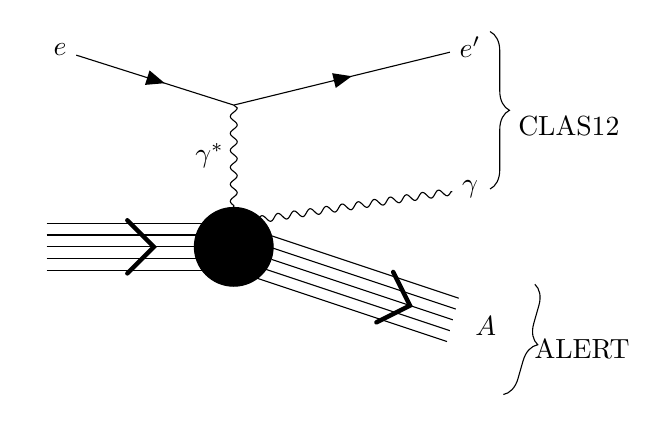
\begin{tikzpicture}[
         nucleon/.style = {thick,fermion},
         deuteron/.style = {double,thick,arrow size=0.5pt, 
         postaction={decorate}, decoration={markings, mark=at position 0.70 
      with {\arrow[scale=0.6]{triangle 45}}}}
]
      \begin{feynman}
         \vertex                                            (n0) {};
         \vertex[large, blob, fill=black,right=2.5cm of n0] (n1) {};

         % incoming A nucleons
         \vertex[above = 0.15cm of n0]  (n01){~};
         \vertex[above = 0.30cm of n0]  (n02){~};
         \vertex[above = 0.45cm of n0]  (n03){~};
         \vertex[below = 0.15cm of n0]  (n04){~};
         \vertex[below = 0.30cm of n0]  (n05){~};
         \vertex[below = 0.45cm of n0]  (n06){~};

         \vertex[above = 0.15cm of n1]  (n11){~};
         \vertex[above = 0.30cm of n1]  (n12){~};
         \vertex[above = 0.45cm of n1]  (n13){~};
         \vertex[below = 0.15cm of n1]  (n14){~};
         \vertex[below = 0.30cm of n1]  (n15){~};
         \vertex[below = 0.45cm of n1]  (n16){~};

         %\vertex[label={[label distance=0.2cm]-130:label},blob, fill=black, 

         \vertex[below right=1.0cm and 3.0cm of n1]            (n2) {};
         \vertex[below right=1.0cm and 3.0cm of n11]  (n21) {};
         \vertex[below right=1.0cm and 3.0cm of n12]  (n22) {};
         \vertex[below right=1.0cm and 3.0cm of n13]  (n23) {};
         \vertex[below right=1.0cm and 3.0cm of n14]  (n24) {};
         \vertex[below right=1.0cm and 3.0cm of n15]  (n25) {};
         \vertex[below right=1.0cm and 3.0cm of n16]  (n26) {};

         \vertex[below right=0.5cm and 1.5cm of n2]      (n3) {};


         % e,e'gamma vertex 
         \vertex[above=1.8cm of n1]                  (q0);

         \vertex[above right=0.5cm and 3.0cm of n1]  (a1);
         \vertex[above=0.0cm of a1]                  (q1){\(\gamma\)};

         % electron
         \vertex[above left=0.5cm and 2.0cm of q0]  (e0) {\(e\)};
         \vertex[above=1.8 of q1]   (e1) {\(e^{\prime}\)};

         \diagram*{
            (e0) -- [fermion] (q0) -- [fermion] (e1),
            (n1) -- [photon, edge label = \(\gamma^{*}\)] (q0),
            (q1) -- [photon] (n12),
            (n01) --  (n11)  --  (n21),
            (n02) --  (n12)  --  (n22),
            %(n03) --  (n13) --  (n23),
            (n04) --  (n14)  --  (n24),
            (n05) --  (n15)  --  (n25),
            %(n06) --  (n16) ,
            (n0) -- [plain,arrow size=6pt, postaction={decorate}, 
            decoration={markings, mark=at position 0.75 with 
         {\arrow[scale=4]{angle 90}}}] (n1) --
         [plain,arrow size=6pt, postaction={decorate}, decoration={markings, 
         mark=at position 0.75 with {\arrow[scale=4]{angle 90}}}] (n2),
         };

         \draw[fill,white,rotate=-15] ($(n2.west)-(0.10cm,0.35cm)$) rectangle 
         ($(n2.west)+(0.10cm,0.35cm)$);
         \vertex[below right=0.01cm and 0.2cm of n2]      (pminus1) {$A$};

         % alert detection
         \draw [decoration={brace,amplitude=7pt}, decorate]
         ($(n2.north east)+(0.7cm,0.4cm)$) -- ++(-0.4cm,-1.4cm);
         \node[] at ($(n2.east)+(1.3cm,-0.3cm)$) {ALERT};

         % CLAS12 detection
         \draw [decoration={brace,amplitude=7pt}, decorate]
         ($(e1.east)+(0.0cm,0.2cm)$) -- ++(-0.0cm,-2.0cm);
         \node[] at ($(e1.east)+(1.0cm,-1.0cm)$) {CLAS12};

      \end{feynman}
   \end{tikzpicture}
\end{center}
\caption{N}
\end{figure}

\begin{figure}
\begin{center}
   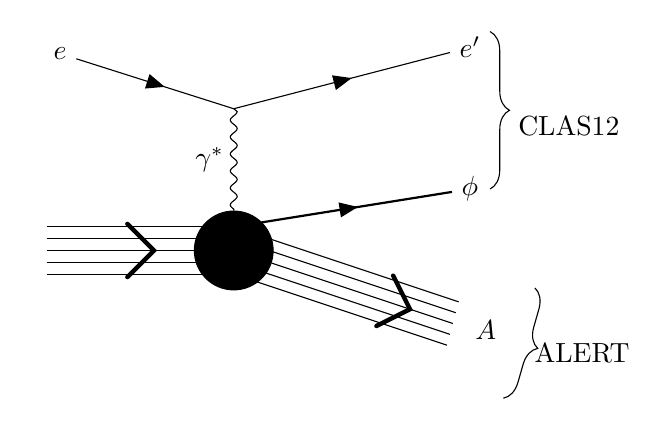
\begin{tikzpicture}[
         nucleon/.style = {thick,fermion},
         deuteron/.style = {double,thick,arrow size=0.5pt, 
         postaction={decorate}, decoration={markings, mark=at position 0.70 
      with {\arrow[scale=0.6]{triangle 45}}}}
]
      \begin{feynman}
         \vertex                                            (n0) {};
         \vertex[large, blob, fill=black,right=2.5cm of n0] (n1) {};

         % incoming A nucleons
         \vertex[above = 0.15cm of n0]  (n01){~};
         \vertex[above = 0.30cm of n0]  (n02){~};
         \vertex[above = 0.45cm of n0]  (n03){~};
         \vertex[below = 0.15cm of n0]  (n04){~};
         \vertex[below = 0.30cm of n0]  (n05){~};
         \vertex[below = 0.45cm of n0]  (n06){~};

         \vertex[above = 0.15cm of n1]  (n11){~};
         \vertex[above = 0.30cm of n1]  (n12){~};
         \vertex[above = 0.45cm of n1]  (n13){~};
         \vertex[below = 0.15cm of n1]  (n14){~};
         \vertex[below = 0.30cm of n1]  (n15){~};
         \vertex[below = 0.45cm of n1]  (n16){~};

         %\vertex[label={[label distance=0.2cm]-130:label},blob, fill=black, 

         \vertex[below right=1.0cm and 3.0cm of n1]            (n2) {};
         \vertex[below right=1.0cm and 3.0cm of n11]  (n21) {};
         \vertex[below right=1.0cm and 3.0cm of n12]  (n22) {};
         \vertex[below right=1.0cm and 3.0cm of n13]  (n23) {};
         \vertex[below right=1.0cm and 3.0cm of n14]  (n24) {};
         \vertex[below right=1.0cm and 3.0cm of n15]  (n25) {};
         \vertex[below right=1.0cm and 3.0cm of n16]  (n26) {};

         \vertex[below right=0.5cm and 1.5cm of n2]      (n3) {};


         % e,e'gamma vertex 
         \vertex[above=1.8cm of n1]                  (q0);

         \vertex[above right=0.5cm and 3.0cm of n1]  (a1);
         \vertex[above=0.0cm of a1]                  (q1){\(\phi\)};

         % electron
         \vertex[above left=0.5cm and 2.0cm of q0]  (e0) {\(e\)};
         \vertex[above=1.8 of q1]   (e1) {\(e^{\prime}\)};

         \diagram*{
            (e0) -- [fermion] (q0) -- [fermion] (e1),
            (n1) -- [photon, edge label = \(\gamma^{*}\)] (q0),
            (n12) -- [thick,fermion] (q1),
            (n01) --  (n11)  --  (n21),
            (n02) --  (n12)  --  (n22),
            %(n03) --  (n13) --  (n23),
            (n04) --  (n14)  --  (n24),
            (n05) --  (n15)  --  (n25),
            %(n06) --  (n16) ,
            (n0) -- [plain,arrow size=6pt, postaction={decorate}, 
            decoration={markings, mark=at position 0.75 with 
         {\arrow[scale=4]{angle 90}}}] (n1) --
         [plain,arrow size=6pt, postaction={decorate}, decoration={markings, 
         mark=at position 0.75 with {\arrow[scale=4]{angle 90}}}] (n2),
         };

         \draw[fill,white,rotate=-15] ($(n2.west)-(0.10cm,0.35cm)$) rectangle 
         ($(n2.west)+(0.10cm,0.35cm)$);
         \vertex[below right=0.01cm and 0.2cm of n2]      (pminus1) {$A$};

         % alert detection
         \draw [decoration={brace,amplitude=7pt}, decorate]
         ($(n2.north east)+(0.7cm,0.4cm)$) -- ++(-0.4cm,-1.4cm);
         \node[] at ($(n2.east)+(1.3cm,-0.3cm)$) {ALERT};

         % CLAS12 detection
         \draw [decoration={brace,amplitude=7pt}, decorate]
         ($(e1.east)+(0.0cm,0.2cm)$) -- ++(-0.0cm,-2.0cm);
         \node[] at ($(e1.east)+(1.0cm,-1.0cm)$) {CLAS12};

      \end{feynman}
   \end{tikzpicture}
\end{center}
\caption{L}
\end{figure}

\begin{figure}
\begin{center}
   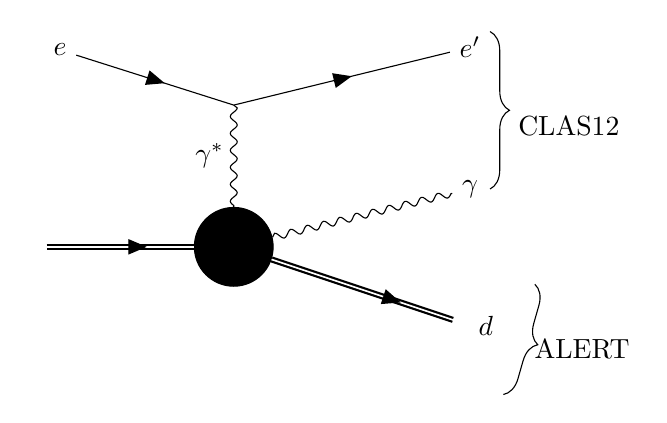
\begin{tikzpicture}[
         nucleon/.style = {thick,fermion},
         deuteron/.style = {double,thick,arrow size=0.5pt, 
         postaction={decorate}, decoration={markings, mark=at position 0.70 
      with {\arrow[scale=0.6]{triangle 45}}}}
]
      \begin{feynman}
         \vertex                                            (n0) {};
         \vertex[large, blob, fill=black,right=2.5cm of n0] (n1) {};
         \vertex[below right=1.0cm and 3.0cm of n1] (n2) {};
         \vertex[below right=0.5cm and 1.5cm of n2] (n3) {};


         % e,e'gamma vertex 
         \vertex[above=1.8cm of n1]                  (q0);

         \vertex[above right=0.5cm and 3.0cm of n1]  (a1);
         \vertex[above=0.0cm of a1]                  (q1){\(\gamma\)};

         % electron
         \vertex[above left=0.5cm and 2.0cm of q0]  (e0) {\(e\)};
         \vertex[above=1.8 of q1]   (e1) {\(e^{\prime}\)};

         \diagram*{
            (e0) -- [fermion] (q0) -- [fermion] (e1),
            (n1) -- [photon, edge label = \(\gamma^{*}\)] (q0),
            (q1) -- [photon] (n1),
            (n0) -- [deuteron] (n1) -- [deuteron] (n2),
         };

         \draw[fill,white,rotate=-15] ($(n2.west)-(0.10cm,0.35cm)$) rectangle 
         ($(n2.west)+(0.10cm,0.35cm)$);
         \vertex[below right=0.01cm and 0.2cm of n2]      (pminus1) {$d$};

         % alert detection
         \draw [decoration={brace,amplitude=7pt}, decorate]
         ($(n2.north east)+(0.7cm,0.4cm)$) -- ++(-0.4cm,-1.4cm);
         \node[] at ($(n2.east)+(1.3cm,-0.3cm)$) {ALERT};

         % CLAS12 detection
         \draw [decoration={brace,amplitude=7pt}, decorate]
         ($(e1.east)+(0.0cm,0.2cm)$) -- ++(-0.0cm,-2.0cm);
         \node[] at ($(e1.east)+(1.0cm,-1.0cm)$) {CLAS12};

      \end{feynman}
   \end{tikzpicture}
\end{center}
\caption{O}
\end{figure}

\clearpage 

\begin{figure}
\begin{center}
   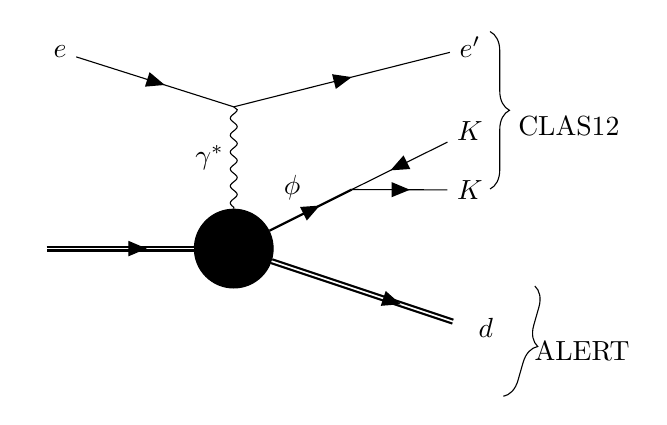
\begin{tikzpicture}[
         nucleon/.style = {thick,fermion},
         deuteron/.style = {double,thick,arrow size=0.5pt, 
         postaction={decorate}, decoration={markings, mark=at position 0.70 
      with {\arrow[scale=0.6]{triangle 45}}}}
]
      \begin{feynman}
         \vertex                                            (n0) {};
         \vertex[large, blob, fill=black,right=2.5cm of n0] (n1) {};
         \vertex[below right=1.0cm and 3.0cm of n1]            (n2) {};
         \vertex[below right=0.5cm and 1.5cm of n2]      (n3) {};

         % e,e'gamma vertex 
         \vertex[above=1.8cm of n1]                  (q0);

         \vertex[above right=0.5cm and 3.0cm of n1]  (a1);
         \vertex[above left=0.25 and 1.5cm of a1]     (q1);
         \vertex[above=0.75cm of a1]                  (pi1){\(K\)};
         \vertex[above=0.0cm of a1]                  (pi2){\(K\)};

         % electron
         \vertex[above left=0.5cm and 2.0cm of q0]  (e0) {\(e\)};
         \vertex[above=1.8 of a1]   (e1) {\(e^{\prime}\)};

         \diagram*{
            (pi1) -- [fermion] (q1) -- [fermion] (pi2),
            (e0) -- [fermion] (q0) -- [fermion] (e1),
            (n1) -- [photon, edge label = \(\gamma^{*}\)] (q0),
            (n1) -- [thick,fermion,edge label = \(\phi\)] (q1),
            (n0) -- [deuteron] (n1) -- [deuteron] (n2),
         };

         \draw[fill,white,rotate=-15] ($(n2.west)-(0.10cm,0.35cm)$) rectangle 
         ($(n2.west)+(0.10cm,0.35cm)$);
         \vertex[below right=0.01cm and 0.2cm of n2]      (pminus1) {$d$};

         % alert detection
         \draw [decoration={brace,amplitude=7pt}, decorate]
         ($(n2.north east)+(0.7cm,0.4cm)$) -- ++(-0.4cm,-1.4cm);
         \node[] at ($(n2.east)+(1.3cm,-0.3cm)$) {ALERT};

         % CLAS12 detection
         \draw [decoration={brace,amplitude=7pt}, decorate]
         ($(e1.east)+(0.0cm,0.2cm)$) -- ++(-0.0cm,-2.0cm);
         \node[] at ($(e1.east)+(1.0cm,-1.0cm)$) {CLAS12};

      \end{feynman}
   \end{tikzpicture}
\end{center}
\caption{P}
\end{figure}

\begin{figure}
\begin{center}
   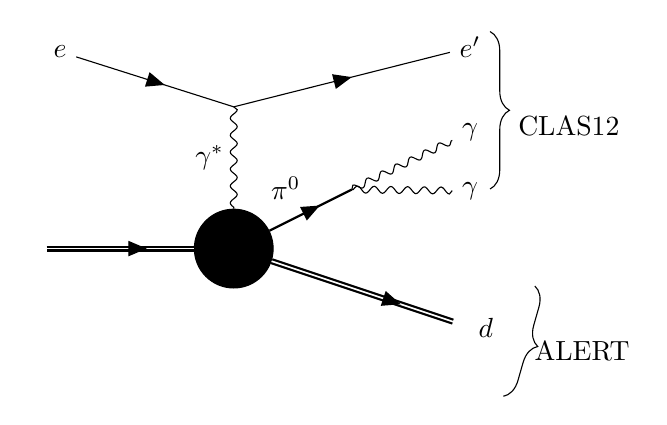
\begin{tikzpicture}[
         nucleon/.style = {thick,fermion},
         deuteron/.style = {double,thick,arrow size=0.5pt, 
         postaction={decorate}, decoration={markings, mark=at position 0.70 
      with {\arrow[scale=0.6]{triangle 45}}}}
]
      \begin{feynman}
         \vertex                                            (n0) {};
         \vertex[large, blob, fill=black,right=2.5cm of n0] (n1) {};
         \vertex[below right=1.0cm and 3.0cm of n1]            (n2) {};
         \vertex[below right=0.5cm and 1.5cm of n2]      (n3) {};

         % e,e'gamma vertex 
         \vertex[above=1.8cm of n1]                  (q0);

         \vertex[above right=0.5cm and 3.0cm of n1]  (a1);
         \vertex[above left=0.25 and 1.5cm of a1]     (q1);
         \vertex[above=0.75cm of a1]                  (pi1){\(\gamma\)};
         \vertex[above=0.0cm of a1]                  (pi2){\(\gamma\)};

         % electron
         \vertex[above left=0.5cm and 2.0cm of q0]  (e0) {\(e\)};
         \vertex[above=1.8 of a1]   (e1) {\(e^{\prime}\)};

         \diagram*{
            (pi1) -- [photon] (q1) -- [photon] (pi2),
            (e0) -- [fermion] (q0) -- [fermion] (e1),
            (n1) -- [photon, edge label = \(\gamma^{*}\)] (q0),
            (n1) -- [thick,fermion,edge label = \(\pi^0\)] (q1),
            (n0) -- [deuteron] (n1) -- [deuteron] (n2),
         };

         \draw[fill,white,rotate=-15] ($(n2.west)-(0.10cm,0.35cm)$) rectangle 
         ($(n2.west)+(0.10cm,0.35cm)$);
         \vertex[below right=0.01cm and 0.2cm of n2]      (pminus1) {$d$};

         % alert detection
         \draw [decoration={brace,amplitude=7pt}, decorate]
         ($(n2.north east)+(0.7cm,0.4cm)$) -- ++(-0.4cm,-1.4cm);
         \node[] at ($(n2.east)+(1.3cm,-0.3cm)$) {ALERT};

         % CLAS12 detection
         \draw [decoration={brace,amplitude=7pt}, decorate]
         ($(e1.east)+(0.0cm,0.2cm)$) -- ++(-0.0cm,-2.0cm);
         \node[] at ($(e1.east)+(1.0cm,-1.0cm)$) {CLAS12};

      \end{feynman}
   \end{tikzpicture}
\end{center}
\caption{P}
\end{figure}

\begin{figure}
\begin{center}
   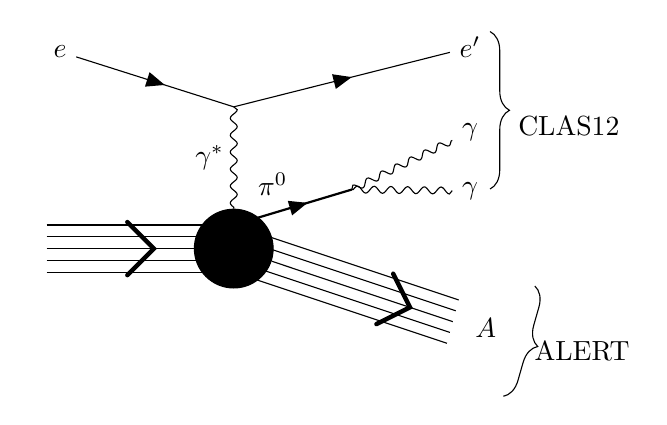
\begin{tikzpicture}[
         nucleon/.style = {thick,fermion},
         deuteron/.style = {double,thick,arrow size=0.5pt, 
         postaction={decorate}, decoration={markings, mark=at position 0.70 
      with {\arrow[scale=0.6]{triangle 45}}}}
]
      \begin{feynman}
         \vertex                                            (n0) {};
         \vertex[large, blob, fill=black,right=2.5cm of n0] (n1) {};

         % incoming A nucleons
         \vertex[above = 0.15cm of n0]  (n01){~};
         \vertex[above = 0.30cm of n0]  (n02){~};
         \vertex[above = 0.45cm of n0]  (n03){~};
         \vertex[below = 0.15cm of n0]  (n04){~};
         \vertex[below = 0.30cm of n0]  (n05){~};
         \vertex[below = 0.45cm of n0]  (n06){~};

         \vertex[above = 0.15cm of n1]  (n11){~};
         \vertex[above = 0.30cm of n1]  (n12){~};
         \vertex[above = 0.45cm of n1]  (n13){~};
         \vertex[below = 0.15cm of n1]  (n14){~};
         \vertex[below = 0.30cm of n1]  (n15){~};
         \vertex[below = 0.45cm of n1]  (n16){~};

         %\vertex[label={[label distance=0.2cm]-130:label},blob, fill=black, 

         \vertex[below right=1.0cm and 3.0cm of n1]            (n2) {};
         \vertex[below right=1.0cm and 3.0cm of n11]  (n21) {};
         \vertex[below right=1.0cm and 3.0cm of n12]  (n22) {};
         \vertex[below right=1.0cm and 3.0cm of n13]  (n23) {};
         \vertex[below right=1.0cm and 3.0cm of n14]  (n24) {};
         \vertex[below right=1.0cm and 3.0cm of n15]  (n25) {};
         \vertex[below right=1.0cm and 3.0cm of n16]  (n26) {};

         \vertex[below right=0.5cm and 1.5cm of n2]      (n3) {};


         % e,e'gamma vertex 
         \vertex[above=1.8cm of n1]                  (q0);

         \vertex[above right=0.5cm and 3.0cm of n1]  (a1);
         \vertex[above right=0.5cm and 3.0cm of n1]  (a11);
         \vertex[above left=0.25 and 1.5cm of a1]     (q1);
         \vertex[above=0.75cm of a1]                  (pi1){\(\gamma\)};
         \vertex[above=0.0cm of a1]                  (pi2){\(\gamma\)};



         % electron
         \vertex[above left=0.5cm and 2.0cm of q0]  (e0) {\(e\)};
         \vertex[above=1.8 of a1]   (e1) {\(e^{\prime}\)};

         \diagram*{
            (pi1) -- [photon] (q1) -- [photon] (pi2),
            (e0) -- [fermion] (q0) -- [fermion] (e1),
            (n1) -- [photon, edge label = \(\gamma^{*}\)] (q0),
            (n12) -- [thick,fermion, edge label = \(\pi^{0}\)] (q1),
            (n01) --  (n11)  --  (n21),
            (n02) --  (n12)  --  (n22),
            %(n03) --  (n13) --  (n23),
            (n04) --  (n14)  --  (n24),
            (n05) --  (n15)  --  (n25),
            %(n06) --  (n16) ,
            (n0) -- [plain,arrow size=6pt, postaction={decorate}, 
            decoration={markings, mark=at position 0.75 with 
         {\arrow[scale=4]{angle 90}}}] (n1) --
         [plain,arrow size=6pt, postaction={decorate}, decoration={markings, 
         mark=at position 0.75 with {\arrow[scale=4]{angle 90}}}] (n2),
         };

         \draw[fill,white,rotate=-15] ($(n2.west)-(0.10cm,0.35cm)$) rectangle 
         ($(n2.west)+(0.10cm,0.35cm)$);
         \vertex[below right=0.01cm and 0.2cm of n2]      (pminus1) {$A$};

         % alert detection
         \draw [decoration={brace,amplitude=7pt}, decorate]
         ($(n2.north east)+(0.7cm,0.4cm)$) -- ++(-0.4cm,-1.4cm);
         \node[] at ($(n2.east)+(1.3cm,-0.3cm)$) {ALERT};

         % CLAS12 detection
         \draw [decoration={brace,amplitude=7pt}, decorate]
         ($(e1.east)+(0.0cm,0.2cm)$) -- ++(-0.0cm,-2.0cm);
         \node[] at ($(e1.east)+(1.0cm,-1.0cm)$) {CLAS12};

      \end{feynman}
   \end{tikzpicture}
\end{center}
\caption{L}
\end{figure}

\begin{figure}
\begin{center}
   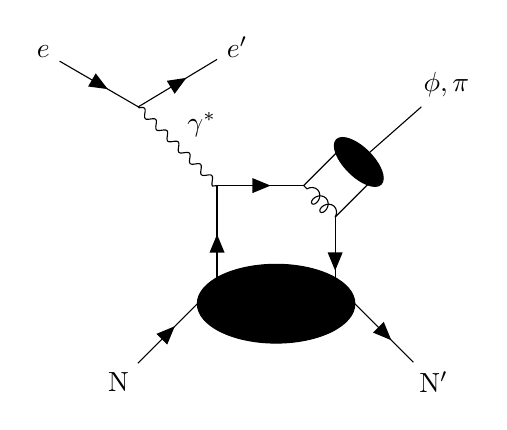
\begin{tikzpicture}
      \begin{feynman}
         \vertex (p1) at (0,0) {N};
         \vertex[above right=1cm and 2.0cm of p1] (a2) { };
         \vertex[below right=1cm and 2.0cm of a2] (p2) {N\(^{\prime}\)};

         \vertex[above left =0.00cm and 1.00cm of a2] (a20);
         \vertex[above left =0.00cm and 0.75cm of a2] (a21);
         \vertex[above left =0.25cm and 0.50cm of a2] (a22);
         \vertex[above left =0.25cm and 0.25cm of a2] (a23);
         \vertex[above right=0.25cm and 0.25cm of a2] (a24);
         \vertex[above right=0.25cm and 0.50cm of a2] (a25);
         \vertex[above right=0.00cm and 0.75cm of a2] (a26);
         \vertex[above right=0.00cm and 1.00cm of a2] (a27);

         \vertex[above =1.5cm of a21] (q0);
         \vertex[above =1.5cm of a26] (q1);


         \vertex[above left =1cm and 1cm of q0] (e0);
         \vertex[above right=1cm and 1cm of q1] (e1){\(\phi, \pi \)};

         \vertex[below=0.4cm of q1] (g1) ;
         \vertex[left=0.4cm of q1] (g2) ;

         \vertex[above right=0.5cm and 0.5cm of g1] (f1);
         \vertex[above right=0.5cm and 0.5cm of g2] (f2);
         \vertex[above right=0.3cm and 0.3cm of q1] (f3);

         \vertex[above left =0.5cm and 1cm of e0] (ee0){\(e\)};
         \vertex[above right=0.5cm and 1cm of e0] (ee1){\(e^{\prime}\)};

         \draw[fill,black] (a2) ellipse (1cm and 0.5cm);
         \diagram* {
            (ee0) -- [fermion] (e0)-- [fermion] (ee1),
            (p1) -- [fermion] (a20),
            (a27) -- [fermion] (p2),
            (a21) -- [fermion] (q0) -- [fermion](g2) -- (f2) -- (f1) -- (g1) -- [fermion](a26),
            (e0) -- [photon, edge label=\(\gamma^{*} \)] (q0),
            (g1) -- [gluon] (g2),
            (f3) -- (e1)
         };

         \draw[fill,black,rotate=45] (f3) ellipse (0.18cm and 0.4cm);

      \end{feynman}
   \end{tikzpicture}
\end{center}
\caption{figure1.pdf}
\end{figure}

\begin{figure}
\begin{center}
   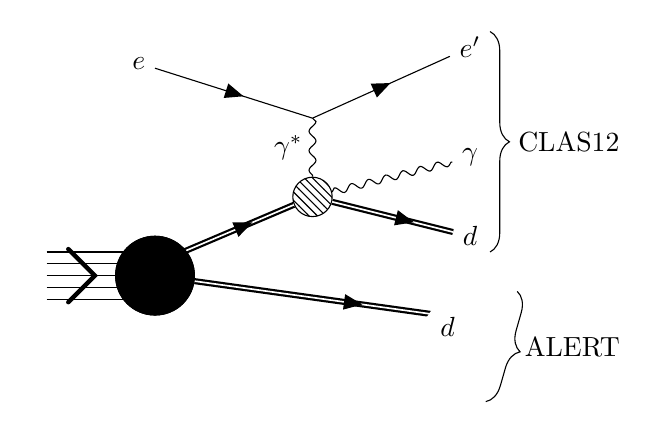
\begin{tikzpicture}[
         nucleon/.style = {thick,fermion},
         deuteron/.style = {double,thick,arrow size=0.5pt, 
         postaction={decorate}, decoration={markings, mark=at position 0.70 
      with {\arrow[scale=0.6]{triangle 45}}}}
]

      \begin{feynman}
         \vertex                                            (n0) {};
         \vertex[large, blob, fill=black,right=1.5cm of n0] (n1) {};

         \vertex[above right=0.6cm and 0.5 of n0]   (Ain) {};

         % incoming A nucleons
         \vertex[above = 0.15cm of n0]  (n01){~};
         \vertex[above = 0.30cm of n0]  (n02){~};
         \vertex[above = 0.45cm of n0]  (n03){~};
         \vertex[below = 0.15cm of n0]  (n04){~};
         \vertex[below = 0.30cm of n0]  (n05){~};
         \vertex[below = 0.45cm of n0]  (n06){~};

         \vertex[above = 0.15cm of n1]  (n11){~};
         \vertex[above = 0.30cm of n1]  (n12){~};
         \vertex[above = 0.45cm of n1]  (n13){~};
         \vertex[below = 0.15cm of n1]  (n14){~};
         \vertex[below = 0.30cm of n1]  (n15){~};
         \vertex[below = 0.45cm of n1]  (n16){~};

         %\vertex[label={[label distance=0.2cm]-130:label},blob, fill=black, 


         \vertex[below right=0.2cm and 2.5cm of n1]   (n2)  ;
         \vertex[below right=0.2cm and 2.55cm of n11]  (n21) ;
         \vertex[below right=0.2cm and 2.45cm of n14]  (n24) ;

         \vertex[below right=0.3cm and 1.1cm of n2]   (n3)  ;
         \vertex[below right=0.8cm and 1.1cm of n21]  (n31) ;
         \vertex[below right=0.8cm and 1.1cm of n24]  (n34) ;


         %dvcs vertex
         \vertex[small, blob, above right=1.0cm and 2.0cm of n1] (a0) {};


         % e,e'gamma vertex 
         \vertex[above=1.0cm of a0]                  (q0);

         \vertex[below right=0.5cm and 2.0cm of a0]  (a1) {$d$};
         \vertex[above=1.0cm of a1]                  (q1){\(\gamma\)};

         % fsi
         \vertex[above right=0.1cm and 2.7cm of n1] (fsi);
         \vertex[left=1.15cm of a1]              (a10);

         % electron
         \vertex[above left=0.5cm and 2.0cm of q0]  (e0) {\(e\)};
         \vertex[above=1.4 of q1]   (e1) {\(e^{\prime}\)};

         \diagram*{
            (e0) -- [fermion] (q0) -- [fermion] (e1),
            (n11) -- [deuteron] (a0),
            (a0)  -- [deuteron] (a1),
            (a0) -- [photon, edge label = \(\gamma^{*}\)] (q0),
            (q1) -- [photon] (a0),
            (n01) --  (n11),%  --  (n21) -- (n31),
            (n02) --  (n12),  %--  (n22),
            %(n03) --  (n13) --  (n23),
            (n04) --  (n14),%  --  (n24) -- (n34),
            (n05) --  (n15),%  --  (n25),
            %(n06) --  (n16) ,
            (n0) -- [plain,arrow size=6pt, postaction={decorate}, 
            decoration={markings, mark=at position 0.75 with 
         {\arrow[scale=4]{angle 90}}}](n1) -- [deuteron](n3),
         %-- [fermion, edge label = \(p_{A-1}\)] (n3),
         };

         %fill in the blob again
         \vertex[large, blob, fill=black,right=1.5cm of n0] {};

         % alert detection
         \draw [decoration={brace,amplitude=7pt}, decorate]
         ($(n3.north east)+(1.0cm,0.3cm)$) -- ++(-0.4cm,-1.4cm);
         \node[] at ($(n3.east)+(1.7cm,-0.4cm)$) {ALERT};

         % CLAS12 detection
         \draw [decoration={brace,amplitude=7pt}, decorate]
         ($(e1.east)+(0.0cm,0.2cm)$) -- ++(-0.0cm,-2.8cm);
         \node[] at ($(e1.east)+(1.0cm,-1.2cm)$) {CLAS12};

         %\draw[fill,black,rotate=-20] (fsi) ellipse (0.18cm and 0.7cm);

         \draw[fill,white,rotate=-35] ($(n3)-(0.10cm,0.3cm)$) rectangle 
         ($(n3)+(0.10cm,0.3cm)$);
         \vertex[below right=-0.1cm and -0.1cm of n3]    (pminus1) {$d$};

      \end{feynman}
   \end{tikzpicture}
\end{center}
\caption{Quasi-coherent deuteron DVCS on He4}
\end{figure}


\begin{figure}
\begin{center}
   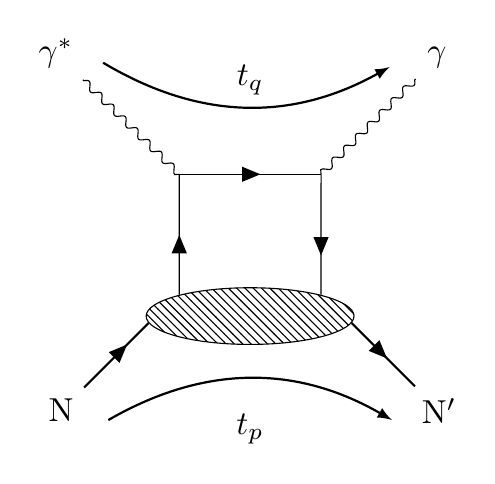
\begin{tikzpicture}[scale=1.2,transform shape,
         nucleon/.style = {thick,fermion},
         deuteron/.style = {double,thick,arrow size=0.5pt, 
         postaction={decorate}, decoration={markings, mark=at position 0.70 
      with {\arrow[scale=0.6]{triangle 45}}}}
]
      \begin{feynman}
         \vertex (p1) at (0,0) {N};
         \vertex[above right=1cm and 2.0cm of p1] (a2) {};
         \vertex[below right=1cm and 2.0cm of a2] (p2) {N\(^{\prime}\)};

         \vertex[above left =0.00cm and 1.00cm of a2] (a20);
         \vertex[above left =0.00cm and 0.75cm of a2] (a21);
         \vertex[above left =0.25cm and 0.50cm of a2] (a22);
         \vertex[above left =0.25cm and 0.25cm of a2] (a23);
         \vertex[above right=0.25cm and 0.25cm of a2] (a24);
         \vertex[above right=0.25cm and 0.50cm of a2] (a25);
         \vertex[above right=0.00cm and 0.75cm of a2] (a26);
         \vertex[above right=0.00cm and 1.00cm of a2] (a27);

         \vertex[above =1.5cm of a21] (q0);
         \vertex[above =1.5cm of a26] (q1);


         \vertex[above left =1cm and 1cm of q0] (e0){\(\gamma^{*}\)};
         \vertex[above right=1cm and 1cm of q1] (e1){\(\gamma \)};

         \vertex[below right =0.1cm and 0.5cm of e0] (t00);
         \vertex[below left  =0.1cm and 0.5cm of e1] (t01);
         %\vertex[above  =2.5cm of a2] (t0) {$t_q=(q_1-q_2)^2$};
         \vertex[above  =2.5cm of a2] (t0) {$t_q$};

         \vertex[below right =0.1cm and 0.5cm of p1] (t10);
         \vertex[below left  =0.1cm and 0.5cm of p2] (t11);
         %\vertex[below =1.5cm of a2] (t1) {$t_p=(p_1-p_2)^2$};
         \vertex[below =1.2cm of a2] (t1) {$t_p$};

         %\vertex[above left =0.5cm and 1cm of e0] (ee0){\(e\)};
         %\vertex[above right=0.5cm and 1cm of e0] (ee1){\(e^{\prime}\)};

         \diagram* {
            (p1) -- [nucleon] (a20),
            (a27) -- [nucleon] (p2),
            (a21) -- [fermion] (q0) -- [fermion](q1) -- [fermion](a26),
            (e0) -- [photon] (q0),
            (e1) -- [photon] (q1),
         };
         \draw[fill,white] (a2) ellipse (1.1cm and 0.3cm);
         \draw[blob] (a2) ellipse (1.1cm and 0.3cm);
         \draw [thick, -latex] (t00) to [bend right] (t01);
         \draw [thick, -latex] (t10) to [bend left] (t11);

      \end{feynman}
   \end{tikzpicture}
\end{center}
\caption{Handbag diagram}
\end{figure}

\begin{figure}
\begin{center}
   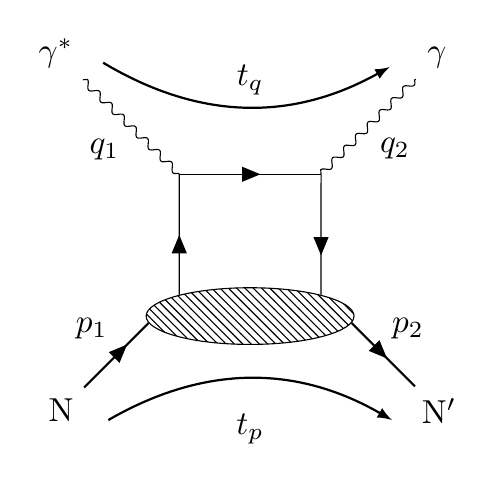
\begin{tikzpicture}[scale=1.2,transform shape,
         nucleon/.style = {thick,fermion},
         deuteron/.style = {double,thick,arrow size=0.5pt, 
         postaction={decorate}, decoration={markings, mark=at position 0.70 
      with {\arrow[scale=0.6]{triangle 45}}}}
]
      \begin{feynman}
         \vertex (p1) at (0,0) {N};
         \vertex[above right=1cm and 2.0cm of p1] (a2) {};
         \vertex[below right=1cm and 2.0cm of a2] (p2) {N\(^{\prime}\)};

         \vertex[above left =0.00cm and 1.00cm of a2] (a20);
         \vertex[above left =0.00cm and 0.75cm of a2] (a21);
         \vertex[above left =0.25cm and 0.50cm of a2] (a22);
         \vertex[above left =0.25cm and 0.25cm of a2] (a23);
         \vertex[above right=0.25cm and 0.25cm of a2] (a24);
         \vertex[above right=0.25cm and 0.50cm of a2] (a25);
         \vertex[above right=0.00cm and 0.75cm of a2] (a26);
         \vertex[above right=0.00cm and 1.00cm of a2] (a27);

         \vertex[above =1.5cm of a21] (q0);
         \vertex[above =1.5cm of a26] (q1);


         \vertex[above left =1cm and 1cm of q0] (e0){\(\gamma^{*}\)};
         \vertex[above right=1cm and 1cm of q1] (e1){\(\gamma \)};

         \vertex[below right =0.1cm and 0.5cm of e0] (t00);
         \vertex[below left  =0.1cm and 0.5cm of e1] (t01);
         %\vertex[above  =2.5cm of a2] (t0) {$t_q=(q_1-q_2)^2$};
         \vertex[above  =2.5cm of a2] (t0) {$t_q$};

         \vertex[below right =0.1cm and 0.5cm of p1] (t10);
         \vertex[below left  =0.1cm and 0.5cm of p2] (t11);
         %\vertex[below =1.5cm of a2] (t1) {$t_p=(p_1-p_2)^2$};
         \vertex[below =1.2cm of a2] (t1) {$t_p$};

         %\vertex[above left =0.5cm and 1cm of e0] (ee0){\(e\)};
         %\vertex[above right=0.5cm and 1cm of e0] (ee1){\(e^{\prime}\)};

         \diagram* {
            (p1) -- [nucleon, edge label = \(p_1\)] (a20),
            (a27) -- [nucleon, edge label = \(p_2\)] (p2),
            (a21) -- [fermion] (q0) -- [fermion](q1) -- [fermion](a26),
            (q0) -- [photon, edge label = \(q_1\)] (e0),
            (e1) -- [photon, edge label = \(q_2\)] (q1),
         };
         \draw[fill,white] (a2) ellipse (1.1cm and 0.3cm);
         \draw[blob] (a2) ellipse (1.1cm and 0.3cm);
         \draw [thick, -latex] (t00) to [bend right] (t01);
         \draw [thick, -latex] (t10) to [bend left] (t11);

      \end{feynman}
   \end{tikzpicture}
\end{center}
\caption{Handbag diagram}
\end{figure}

\begin{figure}
\begin{center}
   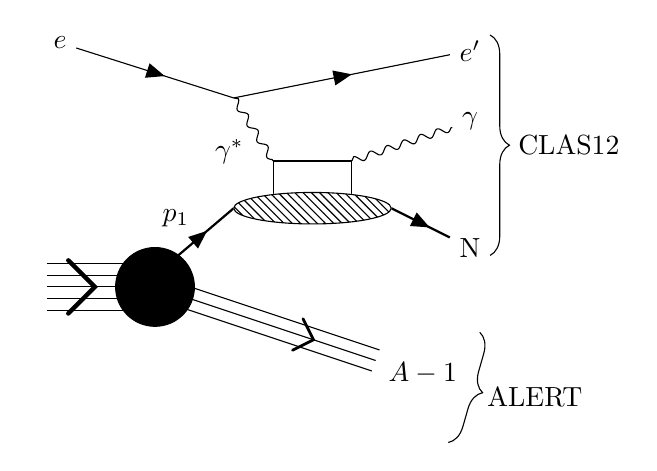
\begin{tikzpicture}
      \begin{feynman}
         \vertex                                            (n0) {};
         \vertex[large, blob, fill=black,right=1.5cm of n0] (n1) {};

         % incoming A nucleons
         \vertex[above = 0.15cm of n0]  (n01){~};
         \vertex[above = 0.30cm of n0]  (n02){~};
         \vertex[above = 0.45cm of n0]  (n03){~};
         \vertex[below = 0.15cm of n0]  (n04){~};
         \vertex[below = 0.30cm of n0]  (n05){~};
         \vertex[below = 0.45cm of n0]  (n06){~};

         \vertex[above = 0.15cm of n1]  (n11){~};
         \vertex[above = 0.30cm of n1]  (n12){~};
         \vertex[above = 0.45cm of n1]  (n13){~};
         \vertex[below = 0.15cm of n1]  (n14){~};
         \vertex[below = 0.30cm of n1]  (n15){~};
         \vertex[below = 0.45cm of n1]  (n16){~};

         \vertex[below right=1.0cm and 3.0cm of n1]            (n2) {};
         %\vertex[label={[label distance=0.2cm]-130:label},blob, fill=black, 

         \vertex[below right=1.0cm and 3.0cm of n11]  (n21) {};
         \vertex[below right=1.0cm and 3.0cm of n12]  (n22) {};
         \vertex[below right=1.0cm and 3.0cm of n13]  (n23) {};
         \vertex[below right=1.0cm and 3.0cm of n14]  (n24) {};
         \vertex[below right=1.0cm and 3.0cm of n15]  (n25) {};
         \vertex[below right=1.0cm and 3.0cm of n16]  (n26) {};

         \vertex[below right=0.5cm and 1.5cm of n2]      (n3) {};

         %dvcs vertex
         \vertex[above right=1.0cm and 2.0cm of n1] (a0) {};
         \coordinate (a00) at ($(a0)-(1,0)$);
         \coordinate (a01) at ($(a0)+(1,0)$);
         \coordinate (a02) at ($(a0)-(0.5,0)$);
         \coordinate (a03) at ($(a0)+(0.5,0)$);
         \coordinate (a04) at ($(a0)-(0.5,0)+(0,0.6)$);
         \coordinate (a05) at ($(a0)+(0.5,0)+(0,0.6)$);

         % e,e'gamma vertex 
         \vertex[above=1.4cm of a00]                  (q0);

         \vertex[below right=0.5cm and 2.0cm of a0]  (a1) {N};
         \vertex[above=1.6cm of a1]                  (q1){\(\gamma\)};

         % fsi
         \node[left=1.15cm of a1]                 (a10);

         % electron
         \vertex[above left=0.5cm and 2.0cm of q0]  (e0) {\(e\)};
         \vertex[above=0.9 of q1]   (e1) {\(e^{\prime}\)};

         \diagram*{
            (e0) -- [fermion] (q0) -- [fermion] (e1), % e-e'
            (n11) -- [thick,fermion, edge label=\(p_1\)] (a00),
            (a01) -- [thick, fermion] (a1),
            (a02) -- [plain] (a04) -- [plain] (a05) -- [plain] (a03), %handbag
            (a04) -- [photon, edge label = \(\gamma^{*}\)] (q0),
            (q1) -- [photon] (a05),
            (n01) --  (n11)  --  (n21),
            (n02) --  (n12),  %--  (n22),
            %(n03) --  (n13) --  (n23),
            (n04) --  (n14)  --  (n24),
            (n05) --  (n15),%  --  (n25),
            %(n06) --  (n16) ,
            (n0) -- [plain,arrow size=6pt, postaction={decorate}, 
            decoration={markings, mark=at position 0.75 with 
         {\arrow[scale=4]{angle 90}}}](n1)
         -- [plain,arrow size=6pt, postaction={decorate}, decoration={markings, 
         mark=at position 0.65 with {\arrow[scale=2.5]{angle 90}}}](n2),
         %-- [fermion, edge label = \(p_{A-1}\)] (n3),
         };

         % alert detection
         \draw [decoration={brace,amplitude=7pt}, decorate]
         ($(n2.north east)+(1.0cm,0.3cm)$) -- ++(-0.4cm,-1.4cm);
         \node[] at ($(n2.east)+(1.7cm,-0.4cm)$) {ALERT};

         % CLAS12 detection
         \draw [decoration={brace,amplitude=7pt}, decorate]
         ($(e1.east)+(0.0cm,0.2cm)$) -- ++(-0.0cm,-2.8cm);
         \node[] at ($(e1.east)+(1.0cm,-1.2cm)$) {CLAS12};

         \draw[fill,white,rotate=-20] ($(n2)-(0.20cm,0.3cm)$) rectangle 
         ($(n2)+(0.20cm,0.3cm)$);
         \vertex[below right=0.1cm and 0.4cm of n2]      (pminus1) {$A-1$};

         \draw[fill,white] (a0) ellipse (1.0cm and 0.2cm);
         \draw[blob] (a0) ellipse (1.0cm and 0.2cm);
      \end{feynman}

   \end{tikzpicture}
\end{center}
\caption{Incoherent DVCS with handbag}
\end{figure}

\begin{figure}
\begin{center}
   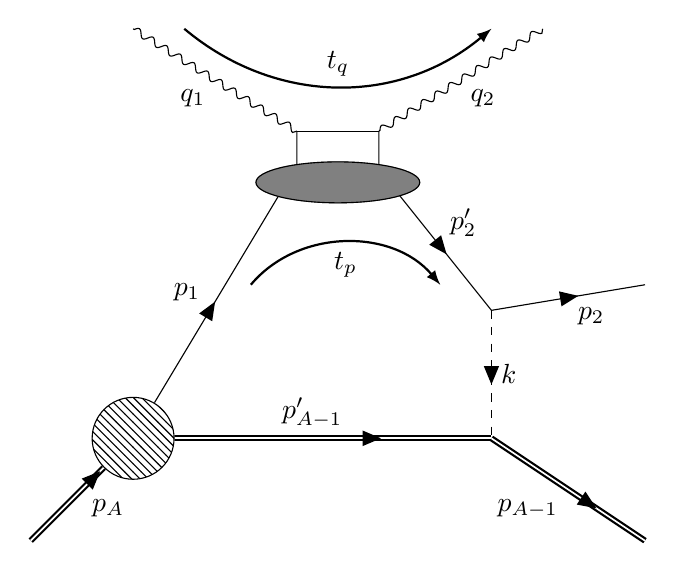
\begin{tikzpicture}[scale=1.3,%transform shape,
         nucleon/.style = {thick,fermion},
         deuteron/.style = {double,thick,arrow size=0.5pt, 
            postaction={decorate}, decoration={markings, mark=at position 0.70 
         with {\arrow[scale=0.6]{triangle 45}}}}
]
      \begin{feynman}
         \vertex (q1) at (-2,2.5);
         \vertex (q2) at ( 2,2.5);
         \vertex (p1) at (-2,-1.5);
         \vertex (p2) at ( 3,0);
         \vertex[blob,fill] (v0) at (0, 1) ;
         \vertex[blob,fill] (v00) at (-0.5, 1) ;
         \vertex[blob,fill] (v01) at ( 0.5, 1) ;
         \vertex (v1)  at (-1,-1.5) ;
         \vertex (v2)  at ( 1.5,-0.25) ;
         \vertex (v20) at ( 1.5,-1.5) ;
         \vertex (pA)  at (-3,-2.5);
         \vertex (pA1) at ( 3,-2.5);
         \vertex (pA11)at ( 3,-2.5);
         \coordinate (hb0)  at ($(v0)-(0.4,0)$);
         \coordinate (hb1)  at ($(v0)+(0.4,0)$);
         \coordinate (hb2)  at ($(hb0)+(0,0.5)$);
         \coordinate (hb3)  at ($(hb1)+(0,0.5)$);

         \diagram*{
            (q1) -- [photon,edge label'=\(q_1\)] (hb2) -- (hb3) -- [photon,edge 
            label'=\(q_2\)] (q2),
            (hb0) -- (hb2) -- (hb3) -- (hb1),
            (p1) -- [fermion,edge label=\(p_1\)] (v00) -- (v01) -- 
            [fermion,edge label=\(p_2^{\prime}\)] (v2)-- [fermion,edge 
            label'=\(p_2\)] (p2),
            (pA) -- [deuteron,edge label'=\(p_{A}\)] (p1) -- [deuteron,edge label=\(p_{A-1}^{\prime}\)] (v20)
            -- [deuteron,edge label'=\(p_{A-1}\)] (pA1),
            (v2) -- [charged scalar,edge label=\(k\)] (v20)
         };
         \draw[fill,gray] (v0) ellipse (0.8cm and 0.2cm);
         \draw[] (v0) ellipse (0.8cm and 0.2cm);

         \draw[fill,white] (p1) ellipse (0.4cm and 0.4cm);
         \draw[blob] (p1) ellipse (0.4cm and 0.4cm);

         \vertex (tq1) at (-1.5,2.5);
         \vertex (tq2) at ( 1.5,2.5);
         \draw [thick, -latex] (tq1) to [bend right=40] node[midway,above] {$t_{q}$} (tq2);

         \vertex (tp1)  at (-0.85,0) ;
         \vertex (tp2)  at ( 1.0,0) ;
         \draw [thick, -latex] (tp1) to [bend left=50] node[midway,below] {$t_{p}$}(tp2);

      \end{feynman}
   \end{tikzpicture}

\end{center}
\caption{FSI with handbag}
\end{figure}

\begin{figure}
\begin{center}
   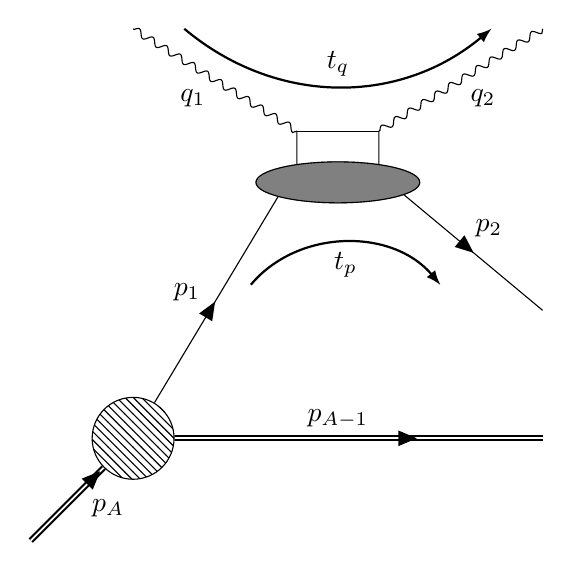
\begin{tikzpicture}[scale=1.3,%transform shape,
         nucleon/.style = {thick,fermion},
         deuteron/.style = {double,thick,arrow size=0.5pt, 
            postaction={decorate}, decoration={markings, mark=at position 0.70 
         with {\arrow[scale=0.6]{triangle 45}}}}
]
      \begin{feynman}
         \vertex (q1) at (-2,2.5);
         \vertex (q2) at ( 2,2.5);
         \vertex (p1) at (-2,-1.5);
         \vertex (p2) at ( 3,0);
         \vertex[blob,fill] (v0) at (0, 1) ;
         \vertex[blob,fill] (v00) at (-0.5, 1) ;
         \vertex[blob,fill] (v01) at ( 0.5, 1) ;
         \vertex (v1)  at (-1,-1.5) ;
         \vertex (v2)  at ( 2.0,-0.25) ;
         \vertex (v20) at ( 2.0,-1.5) ;
         \vertex (pA)  at (-3,-2.5);
         \vertex (pA1) at ( 3,-2.5);
         \vertex (pA11)at ( 3,-2.5);
         \coordinate (hb0)  at ($(v0)-(0.4,0)$);
         \coordinate (hb1)  at ($(v0)+(0.4,0)$);
         \coordinate (hb2)  at ($(hb0)+(0,0.5)$);
         \coordinate (hb3)  at ($(hb1)+(0,0.5)$);

         \diagram*{
            (q1) -- [photon,edge label'=\(q_1\)] (hb2) -- (hb3) -- [photon,edge 
            label'=\(q_2\)] (q2),
            (hb0) -- (hb2) -- (hb3) -- (hb1),
            (p1) -- [fermion,edge label=\(p_1\)] (v00) -- (v01) -- 
            [fermion,edge label=\(p_2\)] (v2), %-- [fermion,edge label'=\(p_2\)] (p2),
            (pA) -- [deuteron,edge label'=\(p_{A}\)] (p1) -- [deuteron,edge 
            label=\(p_{A-1}\)] (v20)%, -- [deuteron,edge label'=\(p_{A-1}\)] (pA1),
            %(v2) -- [charged scalar,edge label=\(k\)] (v20)
         };
         \draw[fill,gray] (v0) ellipse (0.8cm and 0.2cm);
         \draw[] (v0) ellipse (0.8cm and 0.2cm);

         \draw[fill,white] (p1) ellipse (0.4cm and 0.4cm);
         \draw[blob] (p1) ellipse (0.4cm and 0.4cm);

         \vertex (tq1) at (-1.5,2.5);
         \vertex (tq2) at ( 1.5,2.5);
         \draw [thick, -latex] (tq1) to [bend right=40] node[midway,above] {$t_{q}$} (tq2);

         \vertex (tp1)  at (-0.85,0) ;
         \vertex (tp2)  at ( 1.0,0) ;
         \draw [thick, -latex] (tp1) to [bend left=50] node[midway,below] {$t_{p}$}(tp2);

      \end{feynman}
   \end{tikzpicture}

\end{center}
\caption{No FSI with handbag}
\end{figure}

\end{document}



